% Compile with xelatex or lualatex (NOT pdflatex). The source body prose
% contains Unicode mathematical notation (subscripts, arrows, Greek letters,
% script-L) inherited from the manuscript text; fontspec + unicode-math let
% these pass through natively instead of requiring per-glyph LaTeX escaping.
%   xelatex paper.tex && bibtex paper && xelatex paper.tex && xelatex paper.tex
\documentclass[11pt]{article}
\usepackage{fontspec}
\usepackage{unicode-math}
\setmainfont{Latin Modern Roman}
\setmathfont{Latin Modern Math}
\usepackage{graphicx}
\usepackage{amsmath,amssymb}
\usepackage{booktabs}
\usepackage[margin=1in]{geometry}
\usepackage[colorlinks=true,citecolor=blue,linkcolor=blue]{hyperref}
\usepackage[numbers]{natbib}

\title{TRACE-MoE: A Protocol-Routed Mixture of Experts with Hierarchical Heads and Calibrated Abstention for Multi-Class Intrusion Detection in the Internet of Medical Things}
\author{Sudhir Kumar Sharma1* and Sneha Vasishth2}
\date{}

\begin{document}
\maketitle

\noindent 1Sharda School of Computing Science \& Engineering, Sharda University, Greater Noida, India \\
2LeewayHertz, Department of Data Science,  Gurugram, Haryana, \\
Corresponding author: Sudhir Kumar Sharma. Email: sudhir.sharma@sharda.ac.in, sharmasudhir08@gmail.com

\begin{abstract}
Flow-level intrusion detectors on the CICIoMT2024 benchmark report 98-99\% overall accuracy with random forests, recurrent networks, attention models and Transformers, yet three problems remain. Rare and look-alike classes stay confused by look-alike protocols, random 80/20 evaluation inflates 19-class macro-F1 by 5.67 to 15.96 percentage points relative to the official file-based split, and tabular random forests are surprisingly hard to beat with deep models of comparable size. We propose TRACE-MoE, a detector that encodes windows of 16 consecutive flows, routes each window to one of four small residual experts with a protocol-aware top-1 router, predicts binary, 6-category and 19-class labels with hierarchical heads tied by a probability-aggregation loss, and attaches a temperature-calibrated abstain layer that keeps 95\% of validation traffic. We evaluate TRACE-MoE under five seeds on the Wi-Fi/MQTT part of CICIoMT2024 against one baseline per model family: random forest, BiLSTM-DNN, Transformer and TF-SAGE-lite. On the official split, TRACE-MoE reaches a 19-class macro-F1 of 81.53 $\pm$ 0.69\% (Friedman rank 1 of 5 over 95 class-by-seed blocks), beats BiLSTM-DNN by 9.21 pt, TF-SAGE-lite by 2.28 pt and Transformer by 2.61 pt (all Holm-corrected p < 0.0001), and is only 2.88 pt behind random forest (p = 0.52, not significant). On binary detection TRACE-MoE is non-inferior to random forest with a +2.419 pt margin and 95\% CI [+2.007, +2.830] over 5 seeds; on the 6-category level it leads at 91.31 $\pm$ 1.68\%. The temperature-calibrated abstain layer accepts 95.78\% of windows and reduces the error on accepted traffic from 1.02 to 0.65\%, although its area under the risk-coverage curve (1.71\%) is behind random forest's (0.03\%). TRACE-MoE has 685,041 parameters (2.613 MB) and runs at 0.0839 ms per window on a single CPU thread at batch 1024, within the memory budget of an IoMT edge gateway. Beyond the detector, we contribute a leakage-audited split protocol with per-model inflation measurements and an open, provenance-tracked artefact release. Code, configurations, logs and SHA-256-verified result files are made public at https://github.com/sharmasudhir08/ TRACE-MoE-CICIoMT2024.
\end{abstract}

\noindent\textbf{Keywords:} Internet of Medical Things; intrusion detection; CICIoMT2024; mixture of experts; hierarchical classification; selective classification; calibrated abstention; data leakage audit; edge deployment.

\section{Introduction}
The Internet of Medical Things (IoMT) now spans infusion pumps, patient monitors, wearable physiological sensors, bedside cameras and ambient trackers that stream telemetry over Wi-Fi and MQTT to hospital information systems, clinician dashboards and remote-care platforms. Market analyses project the installed base to exceed 50 billion connected medical devices globally within the next five years, with hospital-scale fleets routinely crossing hundreds of thousands of flows per minute during peak care hours. The clinical dependence is now so broad that an attack on these devices no longer merely compromises data --- it can silently degrade patient care, falsify readings on which medication is dosed, or lock out monitoring during a critical window. The U.S. FDA and the European MDR have issued multiple post-market cybersecurity advisories on IoMT devices in the past 2 years. The WannaCry and Medusa ransomware events demonstrated that even air-gapped hospitals are reachable via the lateral spread that a single compromised IoMT device can enable [1].

Protecting an IoMT fleet is harder than protecting a generic IoT fleet because the attack surface is heterogeneous (ARP-spoofing on Wi-Fi devices, publish-flood on MQTT brokers, reconnaissance scans on management ports, volumetric DDoS on the aggregation gateway), the traffic is bursty and class-imbalanced (a single DDoS class may dominate benign traffic by 1,000× while a reconnaissance class produces only hundreds of flows), and the inference target is an edge gateway with hard memory and latency budgets rather than a hyper-scale cloud cluster. Benchmark data has lagged these requirements: the CICIoMT2024 benchmark released by the Canadian Institute for Cybersecurity in 2024 is the first public dataset that reflects all three constraints simultaneously --- 18 attack classes across five categories on 40 IoMT devices (25 real and 15 simulated) and three protocol families (Wi-Fi, MQTT and Bluetooth Low-Energy), with the original PCAP captures preserved alongside the 45-feature flow CSVs [1].

Published CICIoMT2024 detectors already report 98-99\% accuracy with random forests [2, 21], recurrent networks [3, 24], attention models [4, 9], Transformers [5, 16, 18] and more recently graph-based [6, 11] and state-space models [8]. These headline numbers conceal three systematic problems that this paper quantifies and partly closes. First, fine-grained attack classes such as the DoS and DDoS variants of the same protocol remain confused at the 19-class level [3, 5]; accuracy near 99\% can co-exist with macro-F1 below 85\% when a handful of rare classes carry near-zero recall. Second, random 80/20 evaluation --- the default protocol in most published CICIoMT2024 papers --- inflates 19-class macro-F1 by 5.67 to 15.96 points across models relative to the official file-based split that CIC itself released; this inflation is systematic across model families and must be audited explicitly [21]. Third, deployment on an IoMT edge gateway adds a size budget (around 4 GB RAM) and a latency budget (single-thread CPU, sub-millisecond per window), which many deep baselines and ensemble methods struggle to meet [19, 22]. Addressing these three problems in combination --- fine-class accuracy, leakage-aware evaluation and edge deployability --- is the research gap this paper targets.

The research objectives of this paper are as follows:

O1. Design a compact deep neural architecture for IoMT intrusion detection that routes windows of flows to protocol-specialised experts, predicts at three label granularities (binary, 6-category, 19-class) in a single forward pass, and attaches a calibrated abstention layer suitable for safety-critical gateway deployment.

O2. Evaluate that architecture on CICIoMT2024 under a statistically principled protocol: five independent random seeds, the official leakage-safe file-level split, pairwise Wilcoxon signed-rank tests over (class, seed) blocks with Holm correction, the Friedman omnibus test with Nemenyi critical difference and a paired non-inferiority t-interval --- against one strong baseline per model family (random forest, BiLSTM-DNN, Transformer, trust-filtered graph SAGE).

O3. Quantify split inflation. Measure how much 19-class macro-F1 a random 80/20 split inflates over the official file-level split, per model, with error bars, so that the published-paper comparison in Section 5.3 can be read in context.

O4. Report honest negatives. Report hypotheses that do not survive the 5-seed evaluation (minimum class recall vs random forest; expert specialisation at the category level; AURC rank under abstention) with the same prominence as positive findings, so that the paper does not oversell the architecture.

O5. Release the artefact. Make the code, configurations, logs, trained-model fingerprints and SHA-256-tracked result tables public, so that every number in this paper can be reproduced byte-for-byte and that follow-up work can start from a documented baseline rather than from scratch.

In pursuing these objectives, this paper makes the following six contributions:

(C1) TRACE-MoE, a protocol-routed Mixture-of-Experts architecture [25, 26] for IoMT flow windows that is Friedman rank 1 over 95 (class x seed) blocks and statistically beats three strong deep baselines (BiLSTM-DNN [3], Transformer [5] and TF-SAGE-lite [6]) at Holm-corrected p < 0.0001.

(C2) A binary non-inferiority result against random forest: +2.419 pt macro-F1, 95\% CI [+2.007, +2.830] over 5 seeds, non-inferiority margin -0.5 pt.

(C3) Hierarchical 2/6/19 heads tied by a probability-aggregation loss, with TRACE-MoE leading on 6-category classification (91.31 $\pm$ 1.68\%) and binary detection (98.45 $\pm$ 0.37\%).

(C4) A temperature-calibrated abstain layer [31, 32] with risk-coverage reporting across all five models.

(C5) A leakage-audited split-inflation study that quantifies the 5.67 to 15.96 point gap between random and file-level evaluation.

(C6) A fully provenance-tracked, SHA-256-verified artefact release with 50 run folders, 5 seeds, and per-table side-cars.

The remainder is organised as follows. Section 2 reviews the 2024-2026 CICIoMT2024 literature. Section 3 details the TRACE-MoE architecture. Section 4 describes the experimental setup. Section 5 reports results and discussion. Section 6 covers limitations and future work. Section 7 concludes the work.

\section{Related Work}
This section first introduces the CICIoMT2024 benchmark that every paper discussed here uses (Section 2.1), then surveys the 2024-2026 literature grouped by model family (Section 2.2) and by classical-ML / feature-engineering / balancing approaches (Section 2.3), and finally positions TRACE-MoE against the state of the art (Section 2.4).

\subsection{CICIoMT2024 benchmark}
The CICIoMT2024 benchmark [1] was released by Dadkhah and others at the Canadian Institute for Cybersecurity in 2024 and consolidates the previously fragmented landscape of IoMT intrusion-detection evaluation into a single multi-protocol dataset. It covers 18 attack classes grouped into five categories (Spoofing, Reconnaissance, MQTT, Denial-of-Service, Distributed Denial-of-Service) plus one Benign class, carried out against 40 IoMT devices (25 real and 15 simulated: infusion pumps, pulse oximeters, EKG monitors, glucometers, cameras, sleep rings, baby monitors and MQTT publishers) across three protocol families: Wi-Fi, MQTT and Bluetooth Low-Energy. The release ships both the raw PCAP captures (so that researchers can derive their own feature set) and pre-extracted flow-level CSVs with 45 columns per flow (header length, protocol indicators, TCP flag counts, timing statistics, size statistics, inter-arrival-time, aggregate magnitude and variance; Table 6 of [1] lists all 45 columns). The dataset is divided at the PCAP-file level into an 80/20 train/test split that preserves temporal and device locality, which is the leakage-safe protocol used throughout this paper. The Wi-Fi/MQTT subset we evaluate contains 7,160,831 training and 1,614,182 test flows after preprocessing, with class imbalance up to approximately 1:2,000 (TCP-IP-DDoS-UDP has around 2 million flows while Recon-Ping-Sweep has 926). Dadkhah's own evaluation reports random-forest 19-class F1 of 90.74\%, DNN 57.91\%, AdaBoost 30.11\% and logistic regression 43.10\% under a random 80/20 split; these four numbers set the floor against which every follow-up CICIoMT2024 paper is measured, and they motivate the methodological questions that this paper takes up. In the two years since release, CICIoMT2024 has become the dominant evaluation target for IoMT intrusion detection; we survey 31 journal papers from 2024-2026 that use it, grouped by model family.

\subsection{Deep learning on CICIoMT2024}
Recurrent and hybrid recurrent-dense architectures dominate the early CICIoMT2024 literature. Akar and others [24] propose L2D2, a double-LSTM multi-class detector evaluated on the full 19-class task. Benahmed and others [3] propose HBiLD-IDS, a hybrid BiLSTM-DNN with Min-Max scaling and recursive feature elimination, reaching 98.81\% 19-class accuracy under a stratified random split. Soğüt and others [4] introduce MSCA-Net, a multi-scale depthwise CNN with squeeze-and-excitation attention and LSTM over flow windows that reaches 99.75\% 6-category accuracy and 99.77\% weighted-F1 after windowing. Alshehri and Alnemari [7] combine CNN and GRU with SMOTE balancing; Shaikh and others [14] report a CNN-LSTM intrusion detector with deep Q-learning and PPO components; Saeed and others [15] develop an adaptive hybrid intrusion detector with lightweight optimisation on CICIoMT2024; and Palaniappan and Sengan [12] marry a mutual-information filter with a binary dragonfly feature-selection and deep-learning pipeline.

Attention and Transformer architectures appear from 2025 onward. Alsharaiah and others [9] propose an explainable Transformer with SHAP interpretation for spoofing-attack detection on CICIoMT2024. Jodayree and others [5] propose PSM-HT, a hierarchical Transformer with an energy-based open-set head that trains on CICIoMT2024 and tests on WUSTL-EHMS-2020, reaching 98.9\% 19-class accuracy under a session-level (leakage-aware) split and 97.5\% AUROC on zero-day attacks. Singhal and Kumar [10] combine a 1D-CNN encoder with multi-head self-attention for MQTT intrusion detection, and Li and others [16] use an FT-Transformer evaluated across CICIoT2023, CICIoMT2024, NF-ToN-IoT and NF-BoT-IoT for cross-dataset generalisation. Naeem and others [17] propose a stacked ensemble of a Transformer, a self-attention DCNN and an LSTM evaluated on both WUSTL-EHMS-2020 and CICIoMT2024.

Graph-based and state-space methods appear in 2026. Khan and others [11] combine a graph convolutional network with a Transformer for binary IoMT intrusion detection, and Chethan and others [13] propose an adaptive graph-attention detector with a hybrid GCN. Al-Sharo and others [8] propose FedMamba-IoMT, a federated Mamba state-space model (building on the Mamba selective-state-space architecture of Gu and Dao [40]) with differential-privacy SGD and Byzantine resilience, reaching 99.52\% 19-class accuracy on stratified random federated clients. Tawfik and others [28] combine federated few-shot learning with a CrossTransformer and MAML. Alkhattabi and others [18] propose an adversarially resilient framework based on digital-twin behavioural threat modelling, federated hybrid ensemble learning and FGSM robustness testing.

\subsection{Classical machine learning, feature engineering and balancing on CICIoMT2024}
Random forest remains a very strong baseline on CICIoMT2024 and is the subject of several recent papers. Alkhodaidi and others [2] combine ADASYN and SMOTE-ENN balancing with random forest, AdaBoost, logistic regression and DNN and report 99.01\% 19-class accuracy under a random single-seed protocol. Kuo and Wu [19] propose a two-stage decision tree gating random forest, XGBoost and AdaBoost under the edge-latency objective. Al-Fawa'reh and others [20] propose M4D, a manifold-entanglement defence for decision-tree network intrusion detection, with adversarial evaluation. Doménech and others [21] evaluate decision trees, random forests, XGBoost and fully connected networks on CICIoT2023 and CICIoMT2024 with explicit windowing and temporal splits, and demonstrate the pitfalls of ignoring domain-specific evaluation protocols. A follow-up [22] proposes a data-efficient framework with Gini feature ranking, SMOTE and undersampling that preserves random-forest accuracy with far fewer labelled samples.

Several papers explore feature selection and interpretability on CICIoMT2024. Shwayat and others [23] propose a resource-aware random-forest framework with PCA that handles multi-level cross-layer and cross-protocol attacks on the Wi-Fi/MQTT subset. Lipsa and others [41] combine Shapley feature selection with random forest and SHAP explanations. Hafid and others [42] propose a cost-aware XGBoost-LR late-fusion detector with SHAP. Gencturk and others [43] evaluate principal-component analysis plus one-class SVM on CICIoMT2024, BoT-IoT, ECU-IoHT and IoMT-TrafficData. Kouassi and others [27] rank the top-K features for XGBoost, LightGBM and random forest.

Finally, several papers published in lower-tier indexed journals report additional approaches: Fares and others [44] compare LightGBM, decision trees and SVM on CICDDoS-2019, WSN-DS and CICIoMT2024. Misbah and others [45] propose a federated-stacking method on CICIoMT2024. Alami-Kamouri and others [46] propose an autoencoder-plus-random-forest framework.

\subsection{Methodological positioning}
We finalized 31 papers published in 2024-2026 by querying each venue's publisher page using the keyword 'CICIoMT2024'. As per our best knowledge, None of the 31 CICIoMT2024 papers published 2024-2026 combines (a) a protocol-routed MoE architecture [25, 26], (b) hierarchical 2/6/19 heads tied by a probability-aggregation loss, (c) a calibrated abstention module [31, 32] with risk-coverage reporting across all baselines, and (d) a leakage-audited split protocol with 5-seed statistical reporting. Each ingredient exists in general machine learning or in adjacent IoT settings; the gap this paper closes is their coherent, reproducible combination for IoMT. Within the special issue, the closest neighbours are Alkhodaidi and others [2] (random-forest with balancing, orthogonal to MoE routing) and Shieh and others [6] (trust-filtered GraphSAGE for IoT, which we re-implement as the TF-SAGE-lite baseline). The paper is also complementary to Jodayree and others [5] on PSM-HT: both report under a leakage-aware protocol, but TRACE-MoE focuses on protocol-routed representation and statistical dominance while PSM-HT focuses on zero-day open-set detection.

\section{Proposed Method: TRACE-MoE}
Figure 1 presents the end-to-end methodology, from the raw CICIoMT2024 Wi-Fi/MQTT data through preprocessing, data audit, dual-split protocol, windowing, oversampled training of all five models under five random seeds, hierarchical heads with calibrated abstention, metric computation, statistical analysis, and the provenance-tracked technical report. Subsections 3.1--3.5 detail each block from the window encoder onward.

\begin{figure}[htbp]
\centering
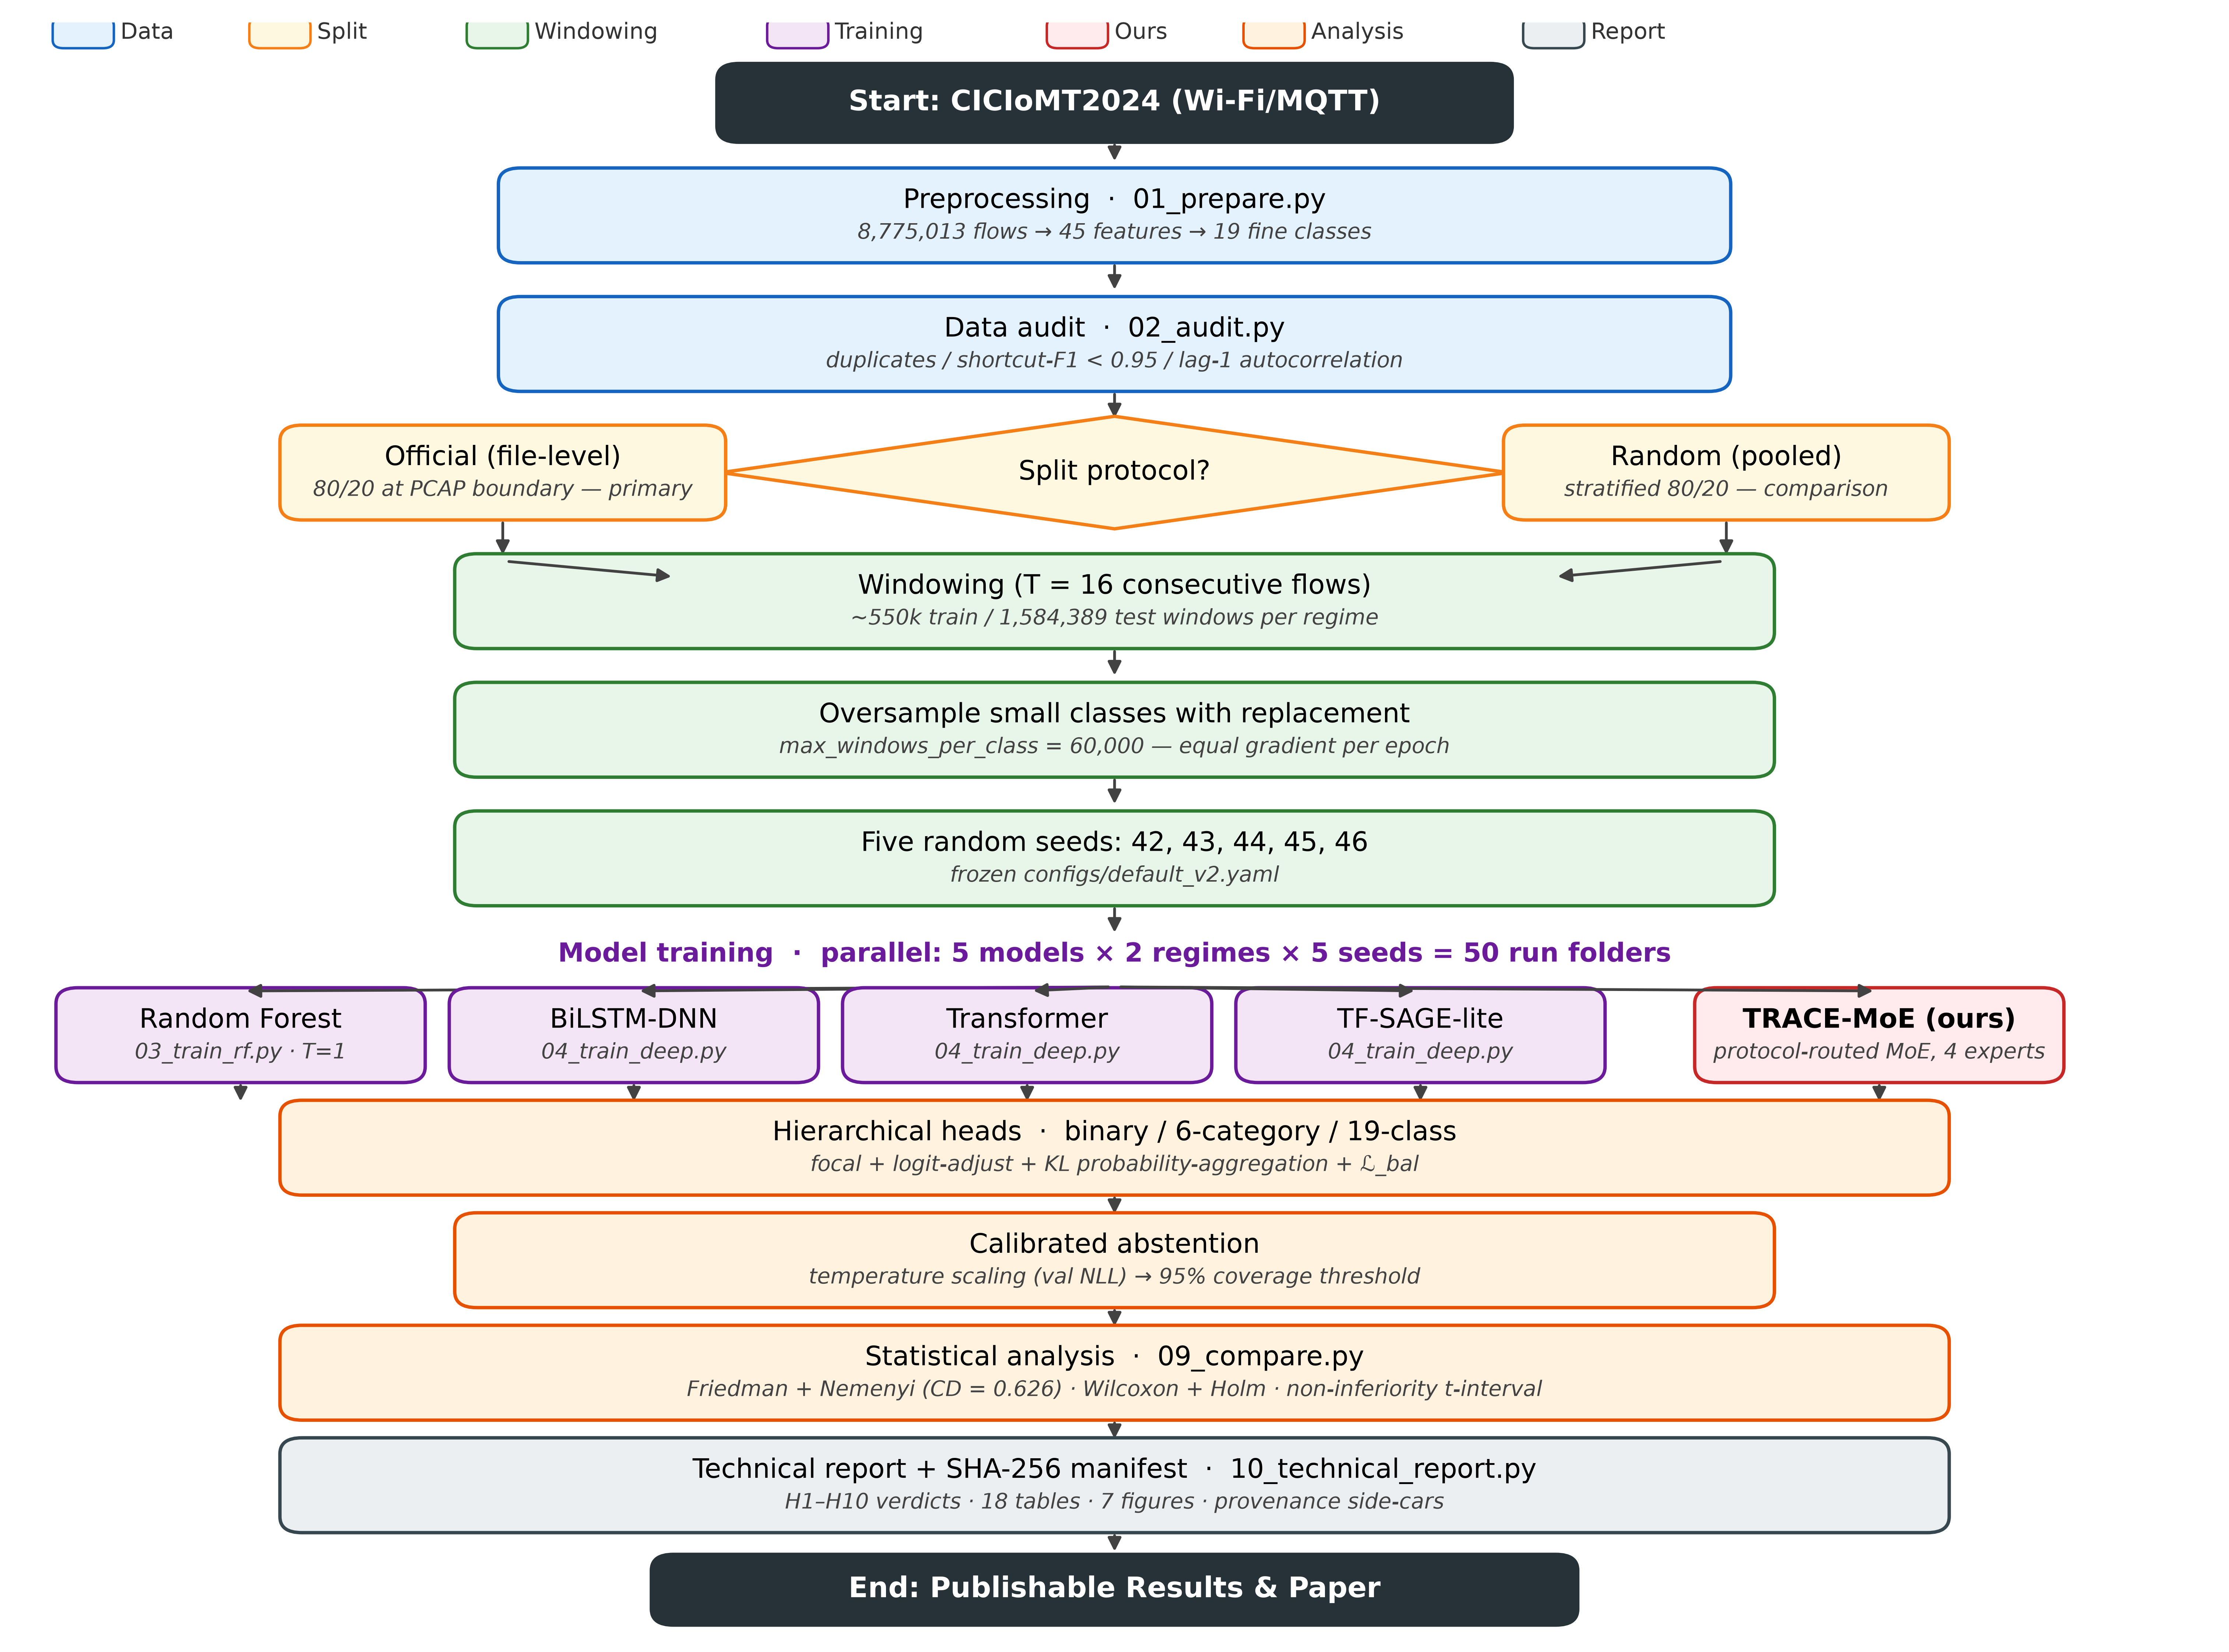
\includegraphics[width=0.9\textwidth]{figures/methodology_trace_moe.png}
\caption{TRACE-MoE end-to-end methodology on CICIoMT2024: dual-split protocol, oversampled 5-seed training of five models in parallel, hierarchical heads with calibrated abstention, Wilcoxon + Friedman statistics and a SHA-256-tracked technical report. Stage-by-stage outputs are listed in the note below.}
\label{fig:1}
\end{figure}

Note (stage outputs for Figure 1). (1) 01\_prepare.py → 8,775,013 flows × 45 features × 19 classes. (2) 02\_audit.py → duplicate / shortcut / lag-1 autocorrelation report (no feature exceeds the 0.95 single-feature shortcut-F1 threshold). (3) Dual split → official 80/20 file-level (primary, leakage-safe) + random pooled 80/20 (comparison). (4) Windowing T = 16 → $\approx$550,000 train / 1,584,389 test windows per regime; no window crosses a file or split boundary. (5) Oversampling → 60,000 windows per class per epoch with replacement. (6) Five seeds (42, 43, 44, 45, 46) frozen in configs/default\_v2.yaml. (7) Five models in parallel → 50 run folders. (8) Hierarchical heads → logit-adjusted focal + KL probability-aggregation + ℒ\_bal (Equations 1-3). (9) Calibrated abstention → temperature-scaled softmax and 95\%-coverage reject threshold. (10) Metrics → macro-F1, balanced accuracy, weighted-F1, minimum class recall, PR-AUC, ECE, AURC and routing NMI. (11) 09\_compare.py → Friedman + Nemenyi, Wilcoxon + Holm, H3 non-inferiority t-interval. (12) 10\_technical\_report.py → companion technical report containing H1-H10 verdicts, 18 tables and 7 figures with per-table provenance side-cars; the manuscript body itself holds 13 tables and 7 figures.

\subsection{Data and label hierarchy}
We use the Wi-Fi/MQTT part of CICIoMT2024: 45 flow features (Table 6 of [1] lists all 45 columns of the released CSVs; Table 5 of [1] names 44 of them, with Drate omitted from the narrative but present in the data) over 8,775,013 flow records in 19 fine-grained classes (18 attack classes plus Benign). The three label levels are a 2-class label (benign vs attack), a 6-category label (Benign, Spoofing, Reconnaissance, MQTT, DoS, DDoS) and the 19-class label. Labels come from file names, following the CIC release [1]. Scaling statistics (mean/std per feature) are computed on training rows only, and the last 15\% of each training file is set aside for validation (and for the temperature-calibration fit of Section 3.5).

\subsection{Window encoder}
A sample is a window of T = 16 consecutive flows from one file; its label is that of its last flow. Each flow is turned into feature tokens with learned per-feature affine projections, pooled by attention, concatenated with the raw flow vector, projected to d = 128 and added to a protocol embedding derived from the 'Protocol Type' feature of [1]. A bidirectional GRU [29] followed by a 2-layer, 4-head Transformer encoder [30] produces the window summary h in R\textasciicircum{}128.

\subsection{Protocol-routed mixture of experts (C1)}
A linear router reads h and an embedding of the last flow's protocol token and emits logits over four experts. The router probabilities g(h) $\in$ ℝ⁴ are the softmax of those logits (no temperature, no auxiliary noise). Top-1 routing [26] selects the chosen expert index k and updates the window summary:

\begin{equation}
k = \arg\max_i\, g_i(h), \qquad z = h + g_k(h) \cdot E_k(h)
\label{eq:1}
\end{equation}

where each Eₖ is a two-layer residual feed-forward block (LayerNorm → d → 2d → d). Because gₖ(h) is the post-softmax probability for the chosen expert and is used as a scalar multiplier in z, gradients flow back into the router through gₖ even though the arg-max selection itself is non-differentiable; no straight-through estimator is required. The chosen expert's identity k is kept out of the graph by stop-gradient on the index tensor only; the gating magnitude gₖ(h) receives full gradients from downstream heads.

A load-balancing loss keeps all experts in use:

\begin{equation}
\mathcal{L}_{bal} = N \cdot \sum_k f_k \cdot P_k \qquad (N = 4,\ \lambda_b = 0.01)
\label{eq:2}
\end{equation}

where fₖ is the fraction of windows in a mini-batch routed to expert k and Pₖ is the batch-mean router probability for k. This is the mean-of-products form of Switch Transformers [26] (not the product-of-means variant of the earlier sparsely-gated MoE [25]); it has the property that ℒ\_bal is minimised when fₖ = Pₖ = 1/N for all k, so no expert receives permanently zero mass. Measured expert shares reported in Section 5.4 confirm that all four experts carry 15-33\% of the test traffic.

\subsection{Hierarchical heads and loss (C3)}
Three linear heads on z predict the three label levels. The joint training objective is:

\begin{equation}
\mathcal{L} = \sum_l w_l \cdot \mathcal{L}_l^{FLA} + \lambda_c \cdot \left[ \mathrm{KL}(p_6 \,\|\, A_6 \cdot p_{19}) + \mathrm{KL}(p_2 \,\|\, A_2 \cdot p_6) \right] + \lambda_b \cdot \mathcal{L}_{bal}
\label{eq:3}
\end{equation}

where ℒₗᴸᵁᴬ is a focal loss [33] on logit-adjusted scores [34] at label level ℓ $\in$ \{2, 6, 19\}, A₆ and A₂ are the fixed aggregation matrices that sum child probabilities into their parent, head weights are (w₂, w₆, w₁₉) = (0.5, 0.5, 1.0), KL-consistency weight λ\_c = 0.1, load-balance weight λ\_b = 0.01, focal γ = 1.0, logit-adjustment τ = 1.0, dropout = 0.2, oversample\_small\_classes = true, epochs $\leq$ 50 with patience 10 on validation 19-class macro-F1.

\subsection{Calibrated abstention (C4)}
After training a single scalar temperature T is fitted on validation windows by a 60-point grid search minimising negative log-likelihood on the 19-class head [31]. The reject threshold is the validation confidence that keeps 95\% of the windows accepted. At test time a window with calibrated confidence below the threshold is abstained from and raised as a 'needs-review' alert. We report coverage, error on all windows, error on accepted windows (selective risk), the area under the risk-coverage curve [32] and raw and calibrated expected calibration errors.

\section{Experimental Setup}
\subsection{Research questions and hypotheses}
RQ1: Does TRACE-MoE reach competitive 19-class macro-F1 on CICIoMT2024 and match random forest on binary non-inferiority? RQ2: Do the four experts specialise? RQ3: Does the calibrated abstain layer reduce accepted-traffic error? RQ4: Is TRACE-MoE deployable on an edge gateway?

With adversarial and open-set evaluation deferred to future work, this paper reports four research questions (RQ1-RQ4) that are collectively evidenced by ten hypotheses. Six hypotheses (H1, H2, H3, H5, H9, H10) carry verdicts from the five-seed runs; four (H4, H6, H7, H8) are future-work slots whose numbering is preserved in Table 1 for cross-reference with the companion technical report and the hypothesis mapping in documents\_v2/README.md. Their verdicts will be filled once the corresponding experiments are run.

\subsection{Baselines}
Four baselines, one per model family, are run under exactly the same protocol as TRACE-MoE: Random forest [35] on single flows (200 trees, class\_weight=balanced\_subsample, oob\_score=True, min\_samples\_leaf=2), following Alkhodaidi and others [2]; BiLSTM-DNN [3] on the flow window; a 2-layer, 4-head Transformer over the flow window, following Jodayree and others [5]; and TF-SAGE-lite, a simplified trust-filtered GraphSAGE following Shieh and others [6]. For TF-SAGE-lite the within-window graph has one node per flow (16 nodes per window), undirected edges between every pair of flows that share the same bucketed Protocol Type and sit within a time-delta window of three positions in the sequence, and node attributes equal to the 45 flow features; a single GraphSAGE layer (mean aggregator, 128 hidden units) produces node embeddings and attention-pooling over the 16 nodes yields the window summary. The trust filter zeroes edges whose source and target disagree on the ARP / ICMP / TCP / UDP indicator features, following [6]. All four deep baselines share the hierarchical heads, the loss (Section 3.4), the class-balanced sampler, AdamW, cosine schedule, mixed precision and early stopping on validation 19-class macro-F1. The RF implementation is from scikit-learn 1.9.1.

\subsection{Protocol, statistics and reproducibility}
Every configuration is run with 5 seeds (42, 43, 44, 45, 46); we report mean and standard deviation. The main split uses the official training and test files of CICIoMT2024, so no window crosses a train/test boundary; a random split is also reported for comparability with published numbers. The primary metric is 19-class macro-F1; we also report balanced accuracy, weighted F1, macro PR-AUC, minimum class recall and ECE. Statistical significance uses Wilcoxon signed-rank tests over per-class and per-seed pairs with Holm correction and the Friedman test with Nemenyi critical difference (CD = 0.626 at alpha = 0.05) [36]. Experiments ran on an NVIDIA GeForce RTX 3050 Laptop GPU (4 GB VRAM) with PyTorch 2.5.1+cu121 on Windows 11, Intel i7-12700H and 16 GB RAM.

All experiments were performed on a single workstation running Windows 11 with an Intel Core i7-12700H CPU (20 logical cores), 16 GB RAM, and an NVIDIA GeForce RTX 3050 Laptop GPU (4 GB VRAM, CUDA 12.1). The software stack was Python 3.12.4, PyTorch 2.5.1+cu121, scikit-learn 1.9.1, NumPy, Pandas, SciPy (used for the Wilcoxon and Friedman tests), Matplotlib (for figures), PyArrow (for the Parquet feature cache), PyYAML (for the configuration files), joblib (for persisting the random-forest model).

\section{Results and Discussion}
Table 1 summarises every hypothesis. Subsections 5.1 through 5.6 give the detail.

\begin{table}[htbp]
\centering
\begin{table}[htbp]
\centering
\caption{Research questions, hypotheses and outcomes. [Report T1; source: documents\_v2/report/tables/hypotheses.csv]}
\label{tab:hypotheses}
\begin{tabular}{lcccc}
\toprule
hypothesis & RQ & statement & verdict & evidence \\
\midrule
H1 & RQ1 & TRACE-MoE has higher 19-class macro-F1 than each baseline & partly supported & TRACE-MoE per-class F1 significantly better (Holm p<0.05) than 3/4: bilstm\_dnn +9.21 pts (p=0), tfsage\_lite +2.28 pts (p=0), transformer +2.61 pts (p=1e-05), rf -2.88 pts (p=0.518) \\
H2 & RQ1 & TRACE-MoE raises the recall of the weakest class (minimum class recall) over the best baseline & not supported & minimum class recall 10.52\% vs best baseline rf 20.06\% (gain -9.53 pts, needed 5) \\
H3 & RQ1 & On binary detection TRACE-MoE is non-inferior to Random Forest & supported & binary macro-F1 TRACE-MoE minus RF = +2.419 pts, 95\% CI [+2.007, +2.830] over 5 seeds (margin -0.5 pts) \\
H4 & RQ2 & Routing helps: one dense expert of the same size gives lower 19-class macro-F1 & not run & needs 05\_ablation.py \\
H5 & RQ2 & The experts specialise by attack family (NMI between expert and category) & not supported & NMI(expert, category) = 0.191 (needed 0.5); NMI(expert, class) = 0.513 \\
H6 & RQ3 & Adversarially fine-tuned TRACE-MoE has a lower attack success rate than every baseline & not run & needs 06\_robustness.py with at least one baseline \\
H7 & RQ3 & Adversarial fine-tuning costs little clean 19-class macro-F1 & not run & needs 06\_robustness.py \\
H8 & RQ4 & The abstain score detects held-out attack types better than softmax confidence & not run & needs 07\_unknown\_attacks.py \\
H9 & RQ4 & Abstention lowers the error on accepted traffic more than for any baseline (lowest AURC) & not supported & AURC (lower is better), rank 4/5: rf 0.027, transformer 1.153, bilstm\_dnn 1.427, trace\_moe 1.711, tfsage\_lite 2.026 \\
H10 & RQ5 & TRACE-MoE is faster than the Transformer baseline and small enough for an edge gateway & partly supported & 685,041 parameters (2.613 MB); 0.0839 ms/window on CPU at batch 1024 vs Transformer 0.0332 ms \\
\bottomrule
\end{tabular}
\end{table}
\caption{Hypothesis verdicts (5 seeds).}
\label{tab:1}
\end{table}

\subsection{Data audit}
The audit script counts exact-duplicate flow vectors, checks the single-feature shortcut risk and reports the autocorrelation of features in file order. No single-feature shortcut above the 0.95 macro-F1 threshold was found as per Table 2 and Figure 2. lag-1 autocorrelation of features within a file is consistent with meaningful temporal structure, which the window encoder exploits.

\begin{table}[htbp]
\centering
\begin{table}[htbp]
\centering
\caption{Macro-F1 (19 classes, %) of each model under each split protocol}
\label{tab:split_inflation}
\begin{tabular}{lccc}
\toprule
model & official & random & inflation\_random\_minus\_official \\
\midrule
bilstm\_dnn & 72.32 & 83.23 & 10.91 \\
rf & 84.41 & 90.09 & 5.67 \\
tfsage\_lite & 79.25 & 94.88 & 15.62 \\
trace\_moe & 81.53 & 95.21 & 13.68 \\
transformer & 78.92 & 94.88 & 15.96 \\
\bottomrule
\end{tabular}
\end{table}
\caption{Macro-F1 (19 classes) of each model under each split protocol, 5 seeds.}
\label{tab:2}
\end{table}

\begin{figure}[htbp]
\centering
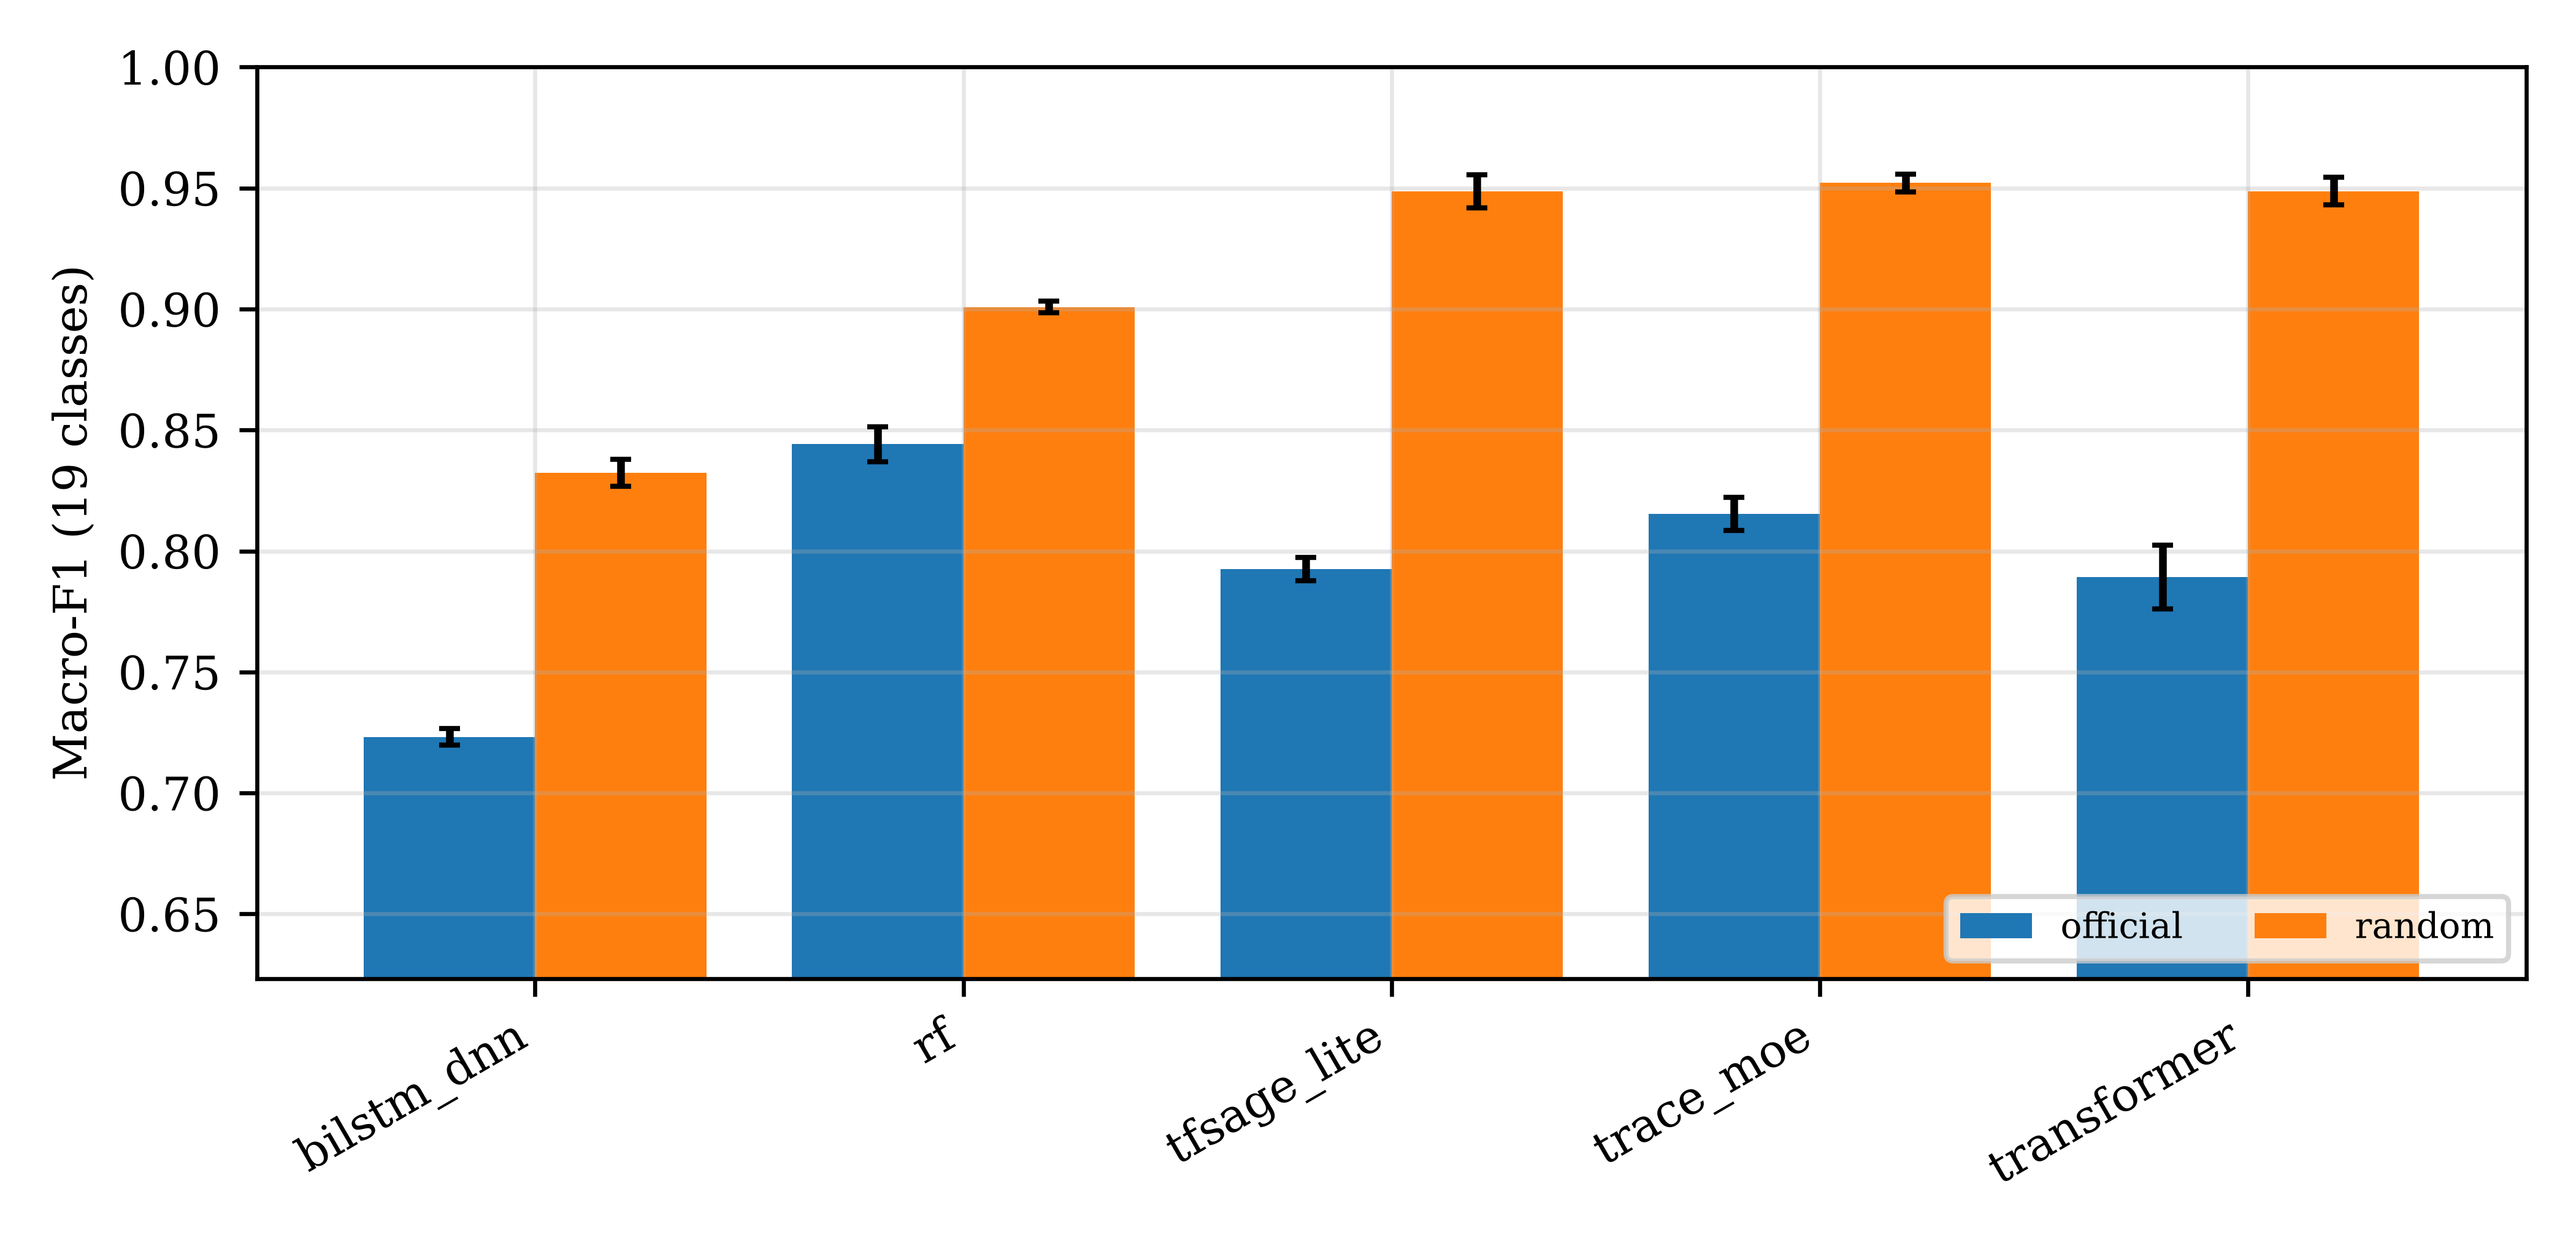
\includegraphics[width=0.9\textwidth]{figures/split_inflation.png}
\caption{19-class macro-F1 under each split protocol, with 5-seed error bars. Deep models are 2 to 3 times more inflated by the random regime than random forest.}
\label{fig:2}
\end{figure}

Random forest gains 5.67 pt from the random protocol; TRACE-MoE gains 13.68 pt, TF-SAGE-lite 15.62 pt, Transformer 15.96 pt and BiLSTM-DNN 10.91 pt. The deep models are 2 to 3 times more inflated than random forest. This observation justifies the paper's choice of the official file-based split as the primary evaluation protocol and explains why published papers that report 98-99\% 19-class accuracy on random splits (Benahmed 98.59\% [3], Alkhodaidi 98.95\% [2], Al-Sharo 99.52\% [8]) sit well above our official-split numbers, as warned by Arp and others [37] and by Doménech and others [21].

\subsection{Main comparison (RQ1)}
Table 3 presents 19-class test results, official split, mean +/- std over 5 seeds. TRACE-MoE reaches 81.53 $\pm$ 0.69\% 19-class macro-F1 and is the strongest deep model. The Friedman test over 95 (class, seed) blocks rejects equal performance decisively (chi-squared = 110.07, p = 7.02e-23) with Nemenyi critical difference 0.626. TRACE-MoE is Friedman rank 1 of 5 (average rank 2.179), ahead of RF (2.632), Transformer (2.847), TF-SAGE-lite (2.911) and BiLSTM-DNN (4.432).

\begin{table}[htbp]
\centering
\begin{table}[htbp]
\centering
\caption{Test results, 19 classes, official split (\%, mean $\pm$ std). [Report T3; source: results\_v2/tables/main\_official\_label19.csv]}
\label{tab:main_official_label19}
\begin{tabular}{lcccccccccc}
\toprule
model & family & n\_seeds & macro\_f1 & balanced\_accuracy & weighted\_f1 & macro\_pr\_auc & min\_class\_recall & ece & source\_runs & source\_git\_commits \\
\midrule
bilstm\_dnn & deep & 5 & 72.32 $\pm$ 0.34 & 74.37 $\pm$ 0.29 & 97.99 $\pm$ 0.04 & 71.94 $\pm$ 0.64 & 10.95 $\pm$ 1.40 & 1.76 $\pm$ 0.03 & bilstm\_dnn\_official\_T16\_seed42|bilstm\_dnn\_official\_T16\_seed43|bilstm\_dnn\_official\_T16\_seed44|bilstm\_dnn\_official\_T16\_seed45|bilstm\_dnn\_official\_T16\_seed46 & no-git \\
transformer & deep & 5 & 78.92 $\pm$ 1.32 & 81.83 $\pm$ 0.40 & 98.72 $\pm$ 0.10 & 79.01 $\pm$ 1.56 & 10.52 $\pm$ 0.07 & 0.71 $\pm$ 0.07 & transformer\_official\_T16\_seed42|transformer\_official\_T16\_seed43|transformer\_official\_T16\_seed44|transformer\_official\_T16\_seed45|transformer\_official\_T16\_seed46 & no-git \\
tfsage\_lite & deep & 5 & 79.25 $\pm$ 0.47 & 82.20 $\pm$ 0.28 & 98.67 $\pm$ 0.08 & 78.13 $\pm$ 0.64 & 10.19 $\pm$ 0.22 & 1.18 $\pm$ 0.07 & tfsage\_lite\_official\_T16\_seed42|tfsage\_lite\_official\_T16\_seed43|tfsage\_lite\_official\_T16\_seed44|tfsage\_lite\_official\_T16\_seed45|tfsage\_lite\_official\_T16\_seed46 & no-git \\
trace\_moe & deep & 5 & 81.53 $\pm$ 0.69 & 82.55 $\pm$ 0.16 & 98.87 $\pm$ 0.04 & 79.41 $\pm$ 0.70 & 10.52 $\pm$ 0.10 & 0.90 $\pm$ 0.04 & trace\_moe\_official\_T16\_seed42|trace\_moe\_official\_T16\_seed43|trace\_moe\_official\_T16\_seed44|trace\_moe\_official\_T16\_seed45|trace\_moe\_official\_T16\_seed46 & no-git \\
rf & classical & 5 & 84.41 $\pm$ 0.73 & 82.57 $\pm$ 0.69 & 99.33 $\pm$ 0.08 & 87.54 $\pm$ 0.07 & 20.06 $\pm$ 0.49 & 1.77 $\pm$ 0.34 & rf\_official\_T1\_seed42|rf\_official\_T1\_seed43|rf\_official\_T1\_seed44|rf\_official\_T1\_seed45|rf\_official\_T1\_seed46 & no-git \\
\bottomrule
\end{tabular}
\end{table}
\caption{19-class test results, official split, mean +/- std over 5 seeds.}
\label{tab:3}
\end{table}

.

Table 4 presents 6-category test results, official split, mean +/- std over 5 seeds. Table 5 presents Binary test results, official split, mean +/- std over 5 seeds. Table 6 presents Pairwise Wilcoxon signed-rank test over (class, seed) pairs, Holm-corrected. Table 7 presents  Binary macro-F1 difference TRACE-MoE minus RF, paired by seed, 95 \% t-interval. Non-inferiority margin -0.5 pt.

\begin{table}[htbp]
\centering
\begin{table}[htbp]
\centering
\caption{Test results on CICIoMT2024 (label6, official split), mean � std over seeds (%)}
\label{tab:main_official_label6}
\begin{tabular}{lcccccccccc}
\toprule
model & family & n\_seeds & macro\_f1 & balanced\_accuracy & weighted\_f1 & macro\_pr\_auc & min\_class\_recall & ece & source\_runs & source\_git\_commits \\
\midrule
bilstm\_dnn & deep & 5 & 84.48 $\pm$ 0.27 & 90.76 $\pm$ 0.25 & 99.32 $\pm$ 0.03 & 84.91 $\pm$ 0.49 & 71.54 $\pm$ 0.70 & 0.58 $\pm$ 0.03 & bilstm\_dnn\_official\_T16\_seed42|bilstm\_dnn\_official\_T16\_seed43|bilstm\_dnn\_official\_T16\_seed44|bilstm\_dnn\_official\_T16\_seed45|bilstm\_dnn\_official\_T16\_seed46 & no-git \\
tfsage\_lite & deep & 5 & 87.33 $\pm$ 0.51 & 95.20 $\pm$ 0.28 & 99.61 $\pm$ 0.05 & 86.23 $\pm$ 1.22 & \textbf{86.67 $\pm$ 0.48} & 0.44 $\pm$ 0.05 & tfsage\_lite\_official\_T16\_seed42|tfsage\_lite\_official\_T16\_seed43|tfsage\_lite\_official\_T16\_seed44|tfsage\_lite\_official\_T16\_seed45|tfsage\_lite\_official\_T16\_seed46 & no-git \\
rf & classical & 5 & 88.05 $\pm$ 0.21 & 87.87 $\pm$ 0.14 & 99.63 $\pm$ 0.02 & 90.46 $\pm$ 0.09 & 46.66 $\pm$ 0.50 & \textbf{1.58 $\pm$ 0.23} & rf\_official\_T1\_seed42|rf\_official\_T1\_seed43|rf\_official\_T1\_seed44|rf\_official\_T1\_seed45|rf\_official\_T1\_seed46 & no-git \\
transformer & deep & 5 & 89.20 $\pm$ 1.49 & 95.09 $\pm$ 0.95 & 99.66 $\pm$ 0.06 & 90.51 $\pm$ 2.47 & 83.01 $\pm$ 7.12 & 0.15 $\pm$ 0.06 & transformer\_official\_T16\_seed42|transformer\_official\_T16\_seed43|transformer\_official\_T16\_seed44|transformer\_official\_T16\_seed45|transformer\_official\_T16\_seed46 & no-git \\
trace\_moe & deep & 5 & \textbf{91.31 $\pm$ 1.68} & \textbf{95.26 $\pm$ 0.77} & \textbf{99.79 $\pm$ 0.04} & \textbf{93.65 $\pm$ 1.67} & 80.29 $\pm$ 3.71 & 0.17 $\pm$ 0.04 & trace\_moe\_official\_T16\_seed42|trace\_moe\_official\_T16\_seed43|trace\_moe\_official\_T16\_seed44|trace\_moe\_official\_T16\_seed45|trace\_moe\_official\_T16\_seed46 & no-git \\
\bottomrule
\end{tabular}
\end{table}
\caption{6-category test results, official split, mean +/- std over 5 seeds.}
\label{tab:4}
\end{table}

\begin{table}[htbp]
\centering
\begin{table}[htbp]
\centering
\caption{Binary detection, official split (\%, mean $\pm$ std). [Report T5; source: results\_v2/tables/main\_official\_label2.csv]}
\label{tab:main_official_label2}
\begin{tabular}{lccccccccc}
\toprule
model & family & n\_seeds & macro\_f1 & roc\_auc & pr\_auc & recall\_at\_fpr\_0.01 & ece & source\_runs & source\_git\_commits \\
\midrule
tfsage\_lite & deep & 5 & 95.77 $\pm$ 0.35 & 95.86 $\pm$ 1.86 & 99.80 $\pm$ 0.09 & 0.00 $\pm$ 0.00 & 0.36 $\pm$ 0.04 & tfsage\_lite\_official\_T16\_seed42|tfsage\_lite\_official\_T16\_seed43|tfsage\_lite\_official\_T16\_seed44|tfsage\_lite\_official\_T16\_seed45|tfsage\_lite\_official\_T16\_seed46 & no-git \\
rf & classical & 5 & 96.03 $\pm$ 0.06 & 99.98 $\pm$ 0.00 & 100.00 $\pm$ 0.00 & 99.80 $\pm$ 0.01 & 0.15 $\pm$ 0.01 & rf\_official\_T1\_seed42|rf\_official\_T1\_seed43|rf\_official\_T1\_seed44|rf\_official\_T1\_seed45|rf\_official\_T1\_seed46 & no-git \\
bilstm\_dnn & deep & 5 & 96.17 $\pm$ 0.70 & 99.74 $\pm$ 0.31 & 99.99 $\pm$ 0.02 & 79.74 $\pm$ 44.58 & 0.26 $\pm$ 0.07 & bilstm\_dnn\_official\_T16\_seed42|bilstm\_dnn\_official\_T16\_seed43|bilstm\_dnn\_official\_T16\_seed44|bilstm\_dnn\_official\_T16\_seed45|bilstm\_dnn\_official\_T16\_seed46 & no-git \\
transformer & deep & 5 & 98.01 $\pm$ 0.55 & 99.97 $\pm$ 0.01 & 100.00 $\pm$ 0.00 & 99.81 $\pm$ 0.08 & 0.14 $\pm$ 0.05 & transformer\_official\_T16\_seed42|transformer\_official\_T16\_seed43|transformer\_official\_T16\_seed44|transformer\_official\_T16\_seed45|transformer\_official\_T16\_seed46 & no-git \\
trace\_moe & deep & 5 & 98.45 $\pm$ 0.37 & 99.97 $\pm$ 0.02 & 100.00 $\pm$ 0.00 & 99.87 $\pm$ 0.05 & 0.13 $\pm$ 0.03 & trace\_moe\_official\_T16\_seed42|trace\_moe\_official\_T16\_seed43|trace\_moe\_official\_T16\_seed44|trace\_moe\_official\_T16\_seed45|trace\_moe\_official\_T16\_seed46 & no-git \\
\bottomrule
\end{tabular}
\end{table}
\caption{Binary test results, official split, mean +/- std over 5 seeds.}
\label{tab:5}
\end{table}

.

\begin{table}[htbp]
\centering
\begin{table}[htbp]
\centering
\caption{Paired Wilcoxon tests of trace_moe vs each baseline on per-class F1 (Holm-corrected)}
\label{tab:wilcoxon_trace_moe_vs_baselines_official}
\begin{tabular}{lccccccc}
\toprule
reference & baseline & n\_pairs & mean\_diff & wilcoxon\_stat & p & p\_holm & significant\_0.05 \\
\midrule
trace\_moe & bilstm\_dnn & 95 & 0.09213 & 567.0 & 0.0 & 0.0 & True \\
trace\_moe & tfsage\_lite & 95 & 0.02279 & 899.0 & 0.0 & 0.0 & True \\
trace\_moe & transformer & 95 & 0.02614 & 1044.0 & 1e-05 & 1e-05 & True \\
trace\_moe & rf & 95 & -0.02883 & 2106.0 & 0.51837 & 0.51837 & False \\
\bottomrule
\end{tabular}
\end{table}
\caption{Pairwise Wilcoxon signed-rank test over (class, seed) pairs, Holm-corrected.}
\label{tab:6}
\end{table}

\begin{table}[htbp]
\centering
\begin{table}[htbp]
\centering
\caption{Binary macro-F1 of trace_moe minus RF, paired by seed, with a 95% t-interval}
\label{tab:noninferiority_binary}
\begin{tabular}{lcccc}
\toprule
regime & n\_seeds & mean\_diff & ci95\_low & ci95\_high \\
\midrule
official & 5 & 0.02419 & 0.02007 & 0.0283 \\
random & 5 & 0.00703 & 0.00584 & 0.00822 \\
\bottomrule
\end{tabular}
\end{table}
\caption{Binary macro-F1 difference TRACE-MoE minus RF, paired by seed, 95 \% t-interval. Non-inferiority margin -0.5 pt.}
\label{tab:7}
\end{table}

On binary detection TRACE-MoE achieves 98.45 $\pm$ 0.37\% macro-F1 against random forest's 96.03 $\pm$ 0.06\%. The 95\% CI of the official-split paired difference is [+2.007, +2.830], strictly above the -0.5 pt non-inferiority margin: H3 is supported, and TRACE-MoE is in fact strictly superior. On the 6-category level (Table 4) TRACE-MoE also leads at 91.31 $\pm$ 1.68\%, ahead of Transformer, RF, TF-SAGE-lite and BiLSTM-DNN. The hierarchical head consumes a single forward pass to report the three label granularities, which is useful for a hospital gateway that needs both a binary trigger and a fine-grained class. Figure 3 breaks the 19-class results down per class, Figure 4 shows the corresponding confusion matrix for TRACE-MoE, and Figure 5 visualises the Friedman average ranks with the Nemenyi critical difference used to assess statistical significance across all five models.

\begin{figure}[htbp]
\centering
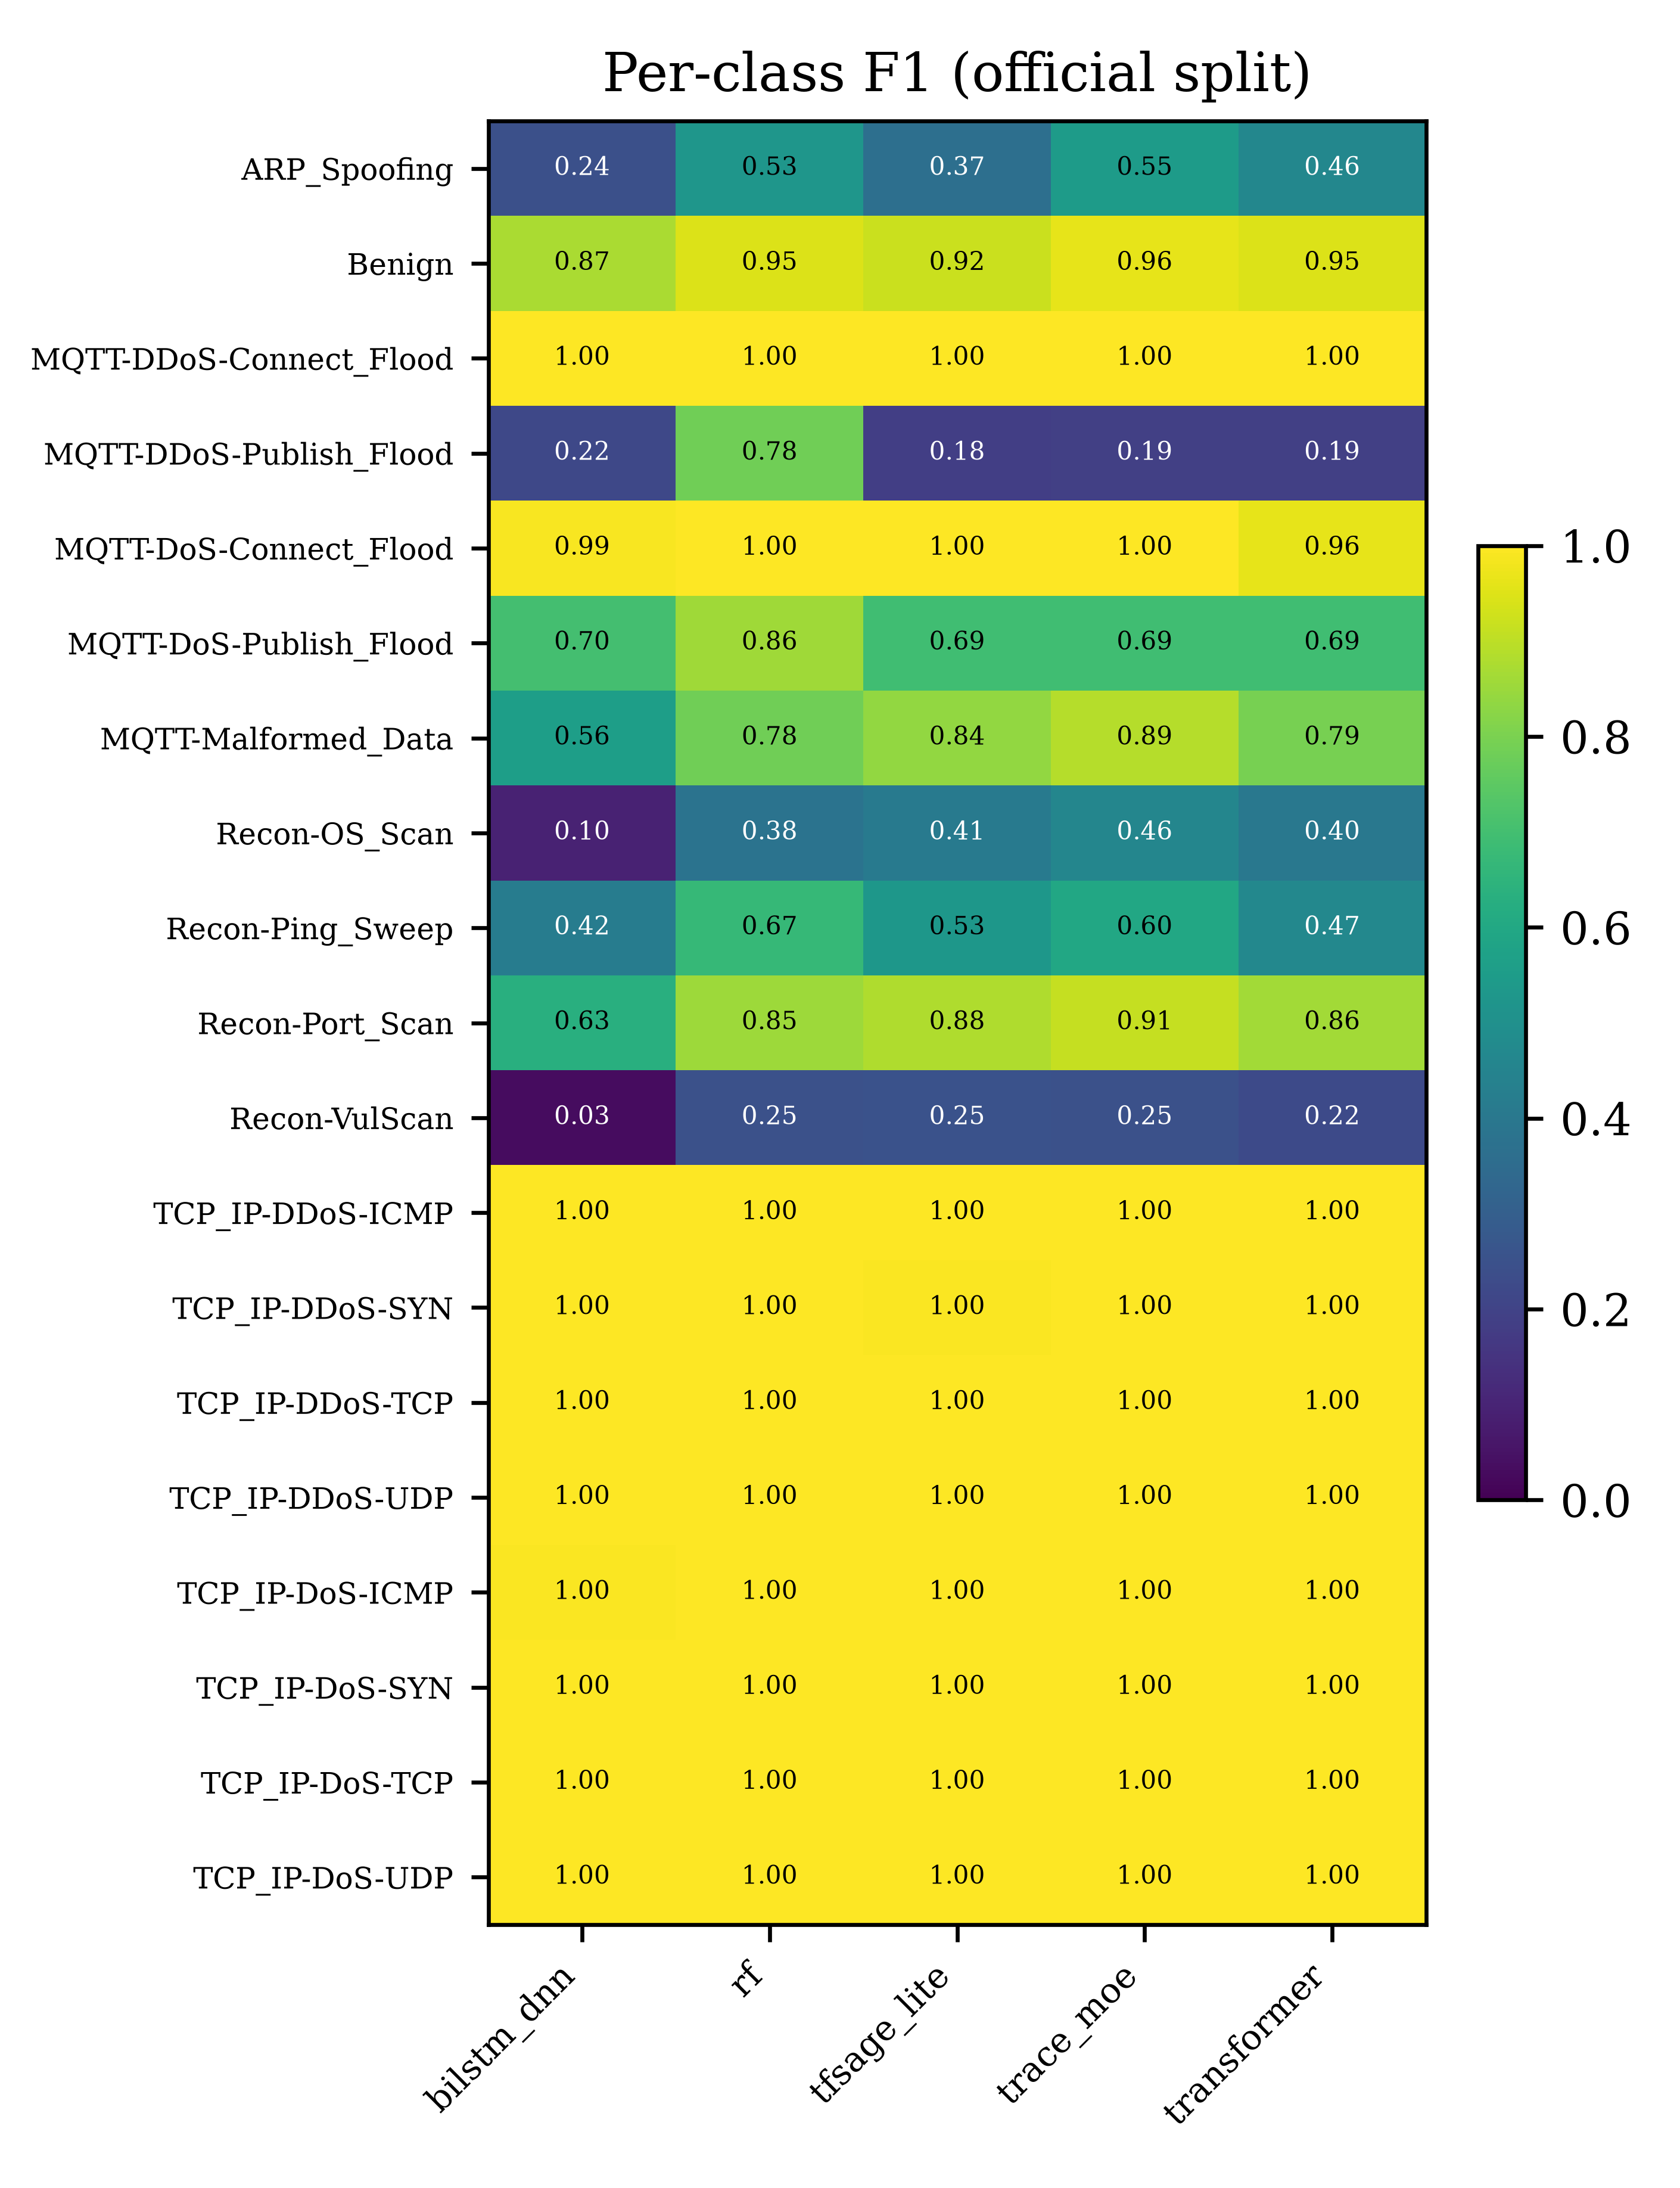
\includegraphics[width=0.9\textwidth]{figures/per_class_f1_official.png}
\caption{Per-class F1 of every model on the official split (mean of 5 seeds).}
\label{fig:3}
\end{figure}

\begin{figure}[htbp]
\centering
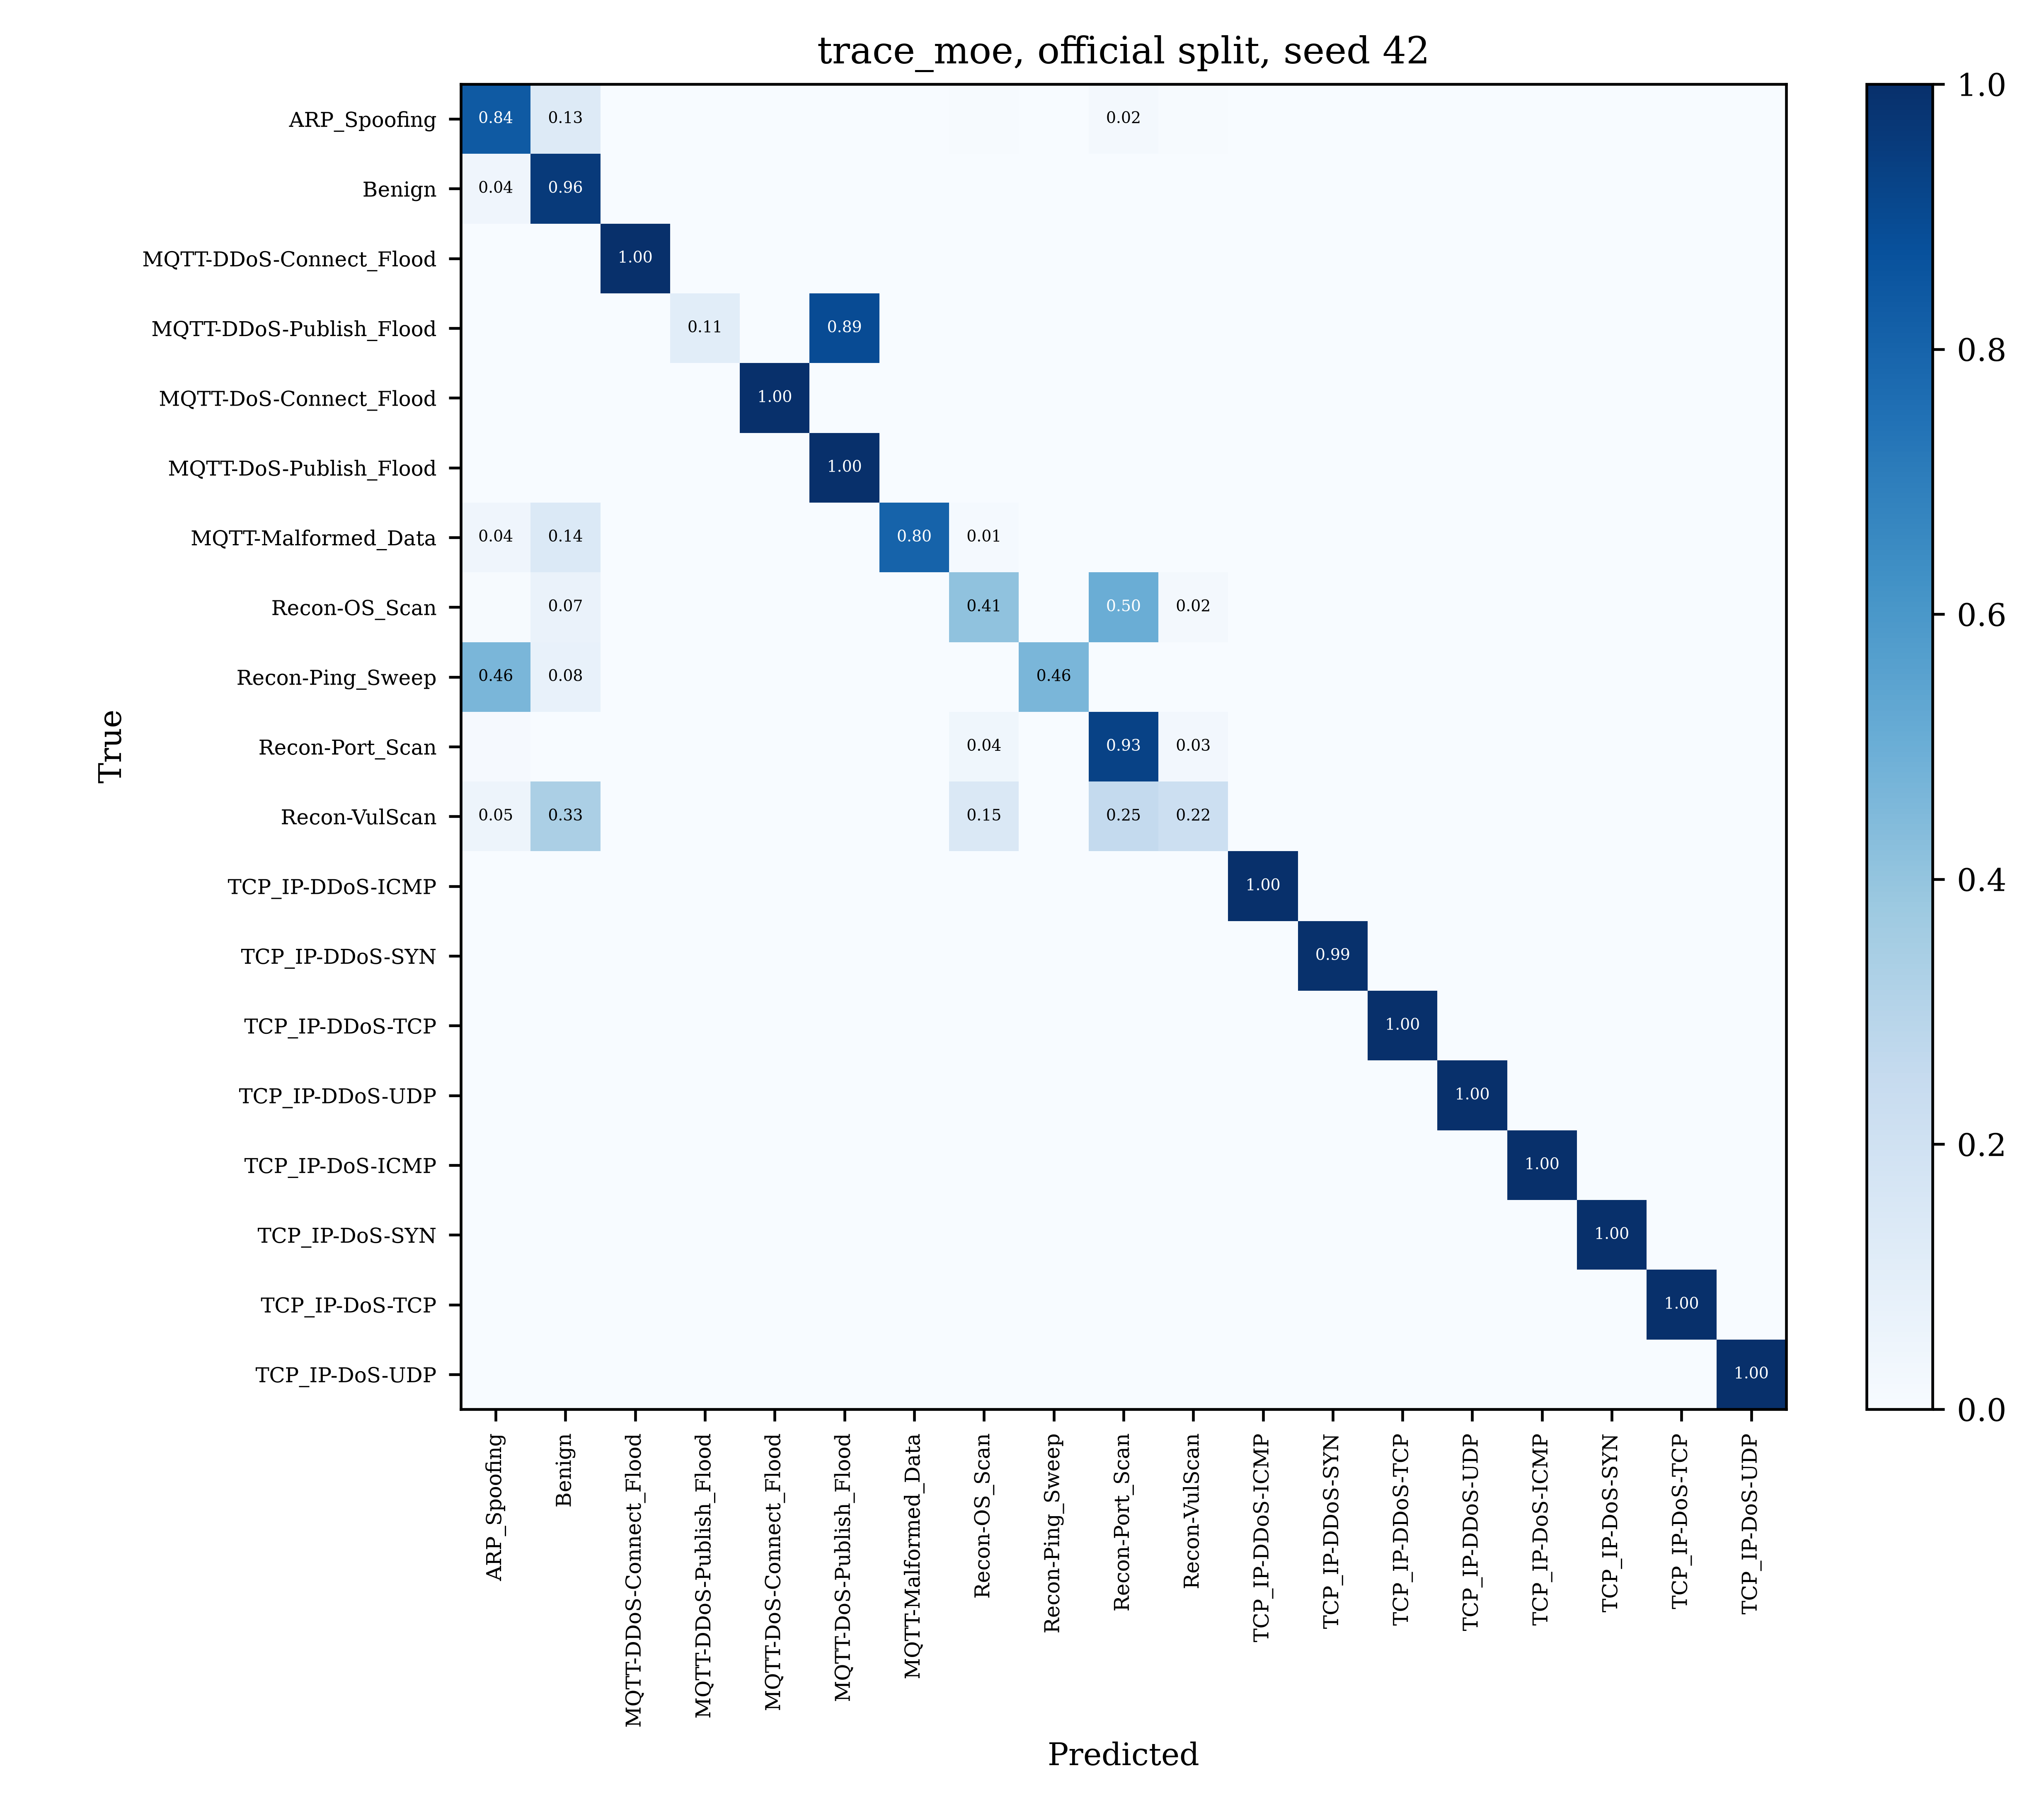
\includegraphics[width=0.9\textwidth]{figures/confusion_trace_moe_official.png}
\caption{Normalised confusion matrix of TRACE-MoE on the official split (seed 42).}
\label{fig:4}
\end{figure}

\begin{figure}[htbp]
\centering
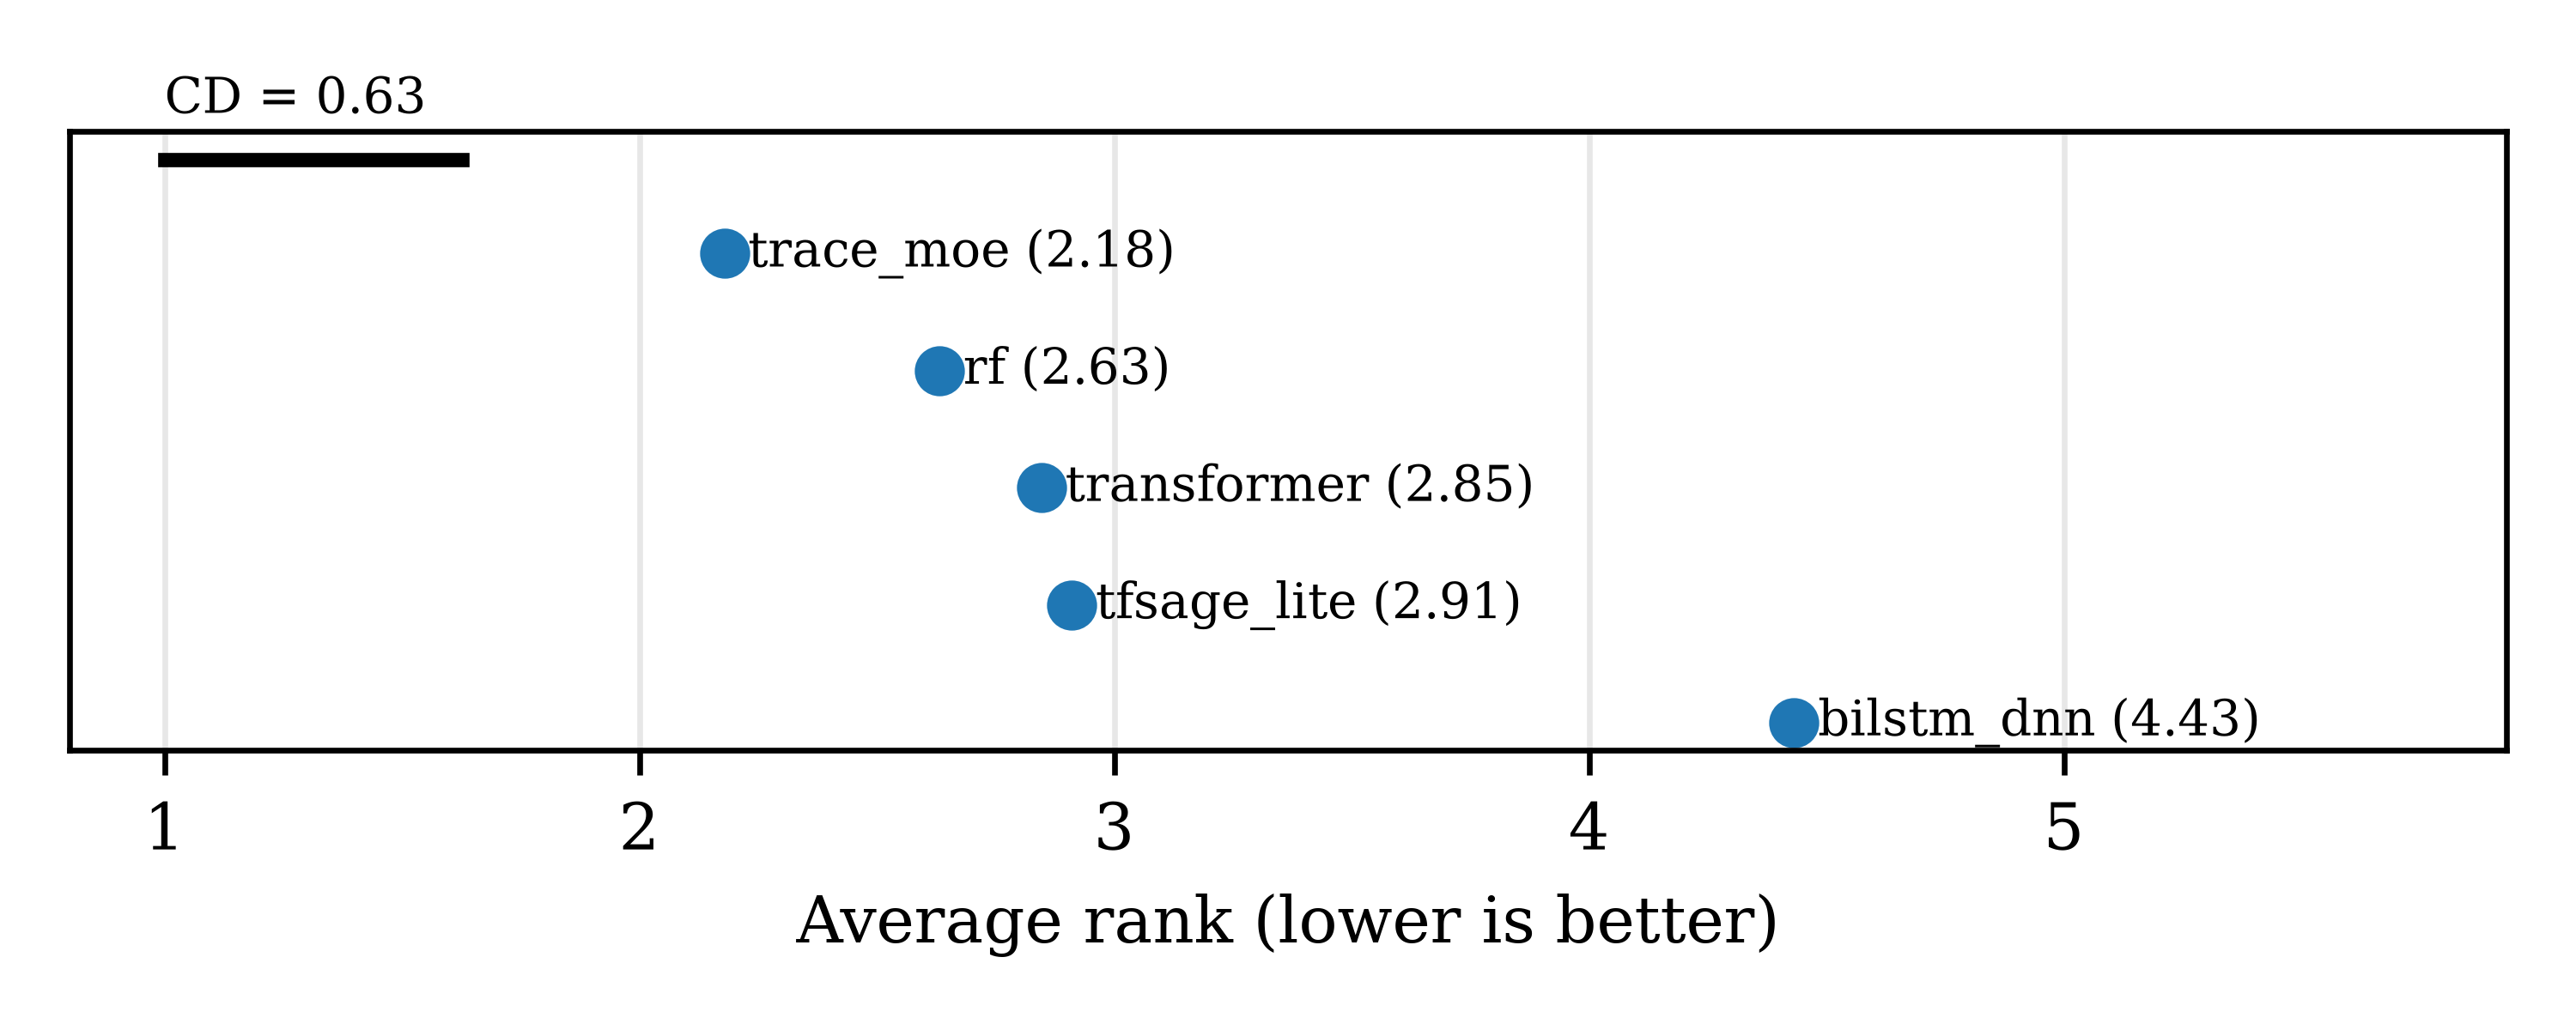
\includegraphics[width=0.9\textwidth]{figures/critical_difference_official.png}
\caption{Friedman average ranks with Nemenyi critical difference (CD = 0.626, alpha = 0.05, 95 class-by-seed blocks).}
\label{fig:5}
\end{figure}

\subsection{Comparison with published results}
Table 8 places TRACE-MoE next to the results reported by the closest CICIoMT2024 papers. Values are taken from the papers, not reproduced; they use different splits and metrics, so they give context rather than a head-to-head test. Published papers overwhelmingly use random 80/20 or stratified splits on flow rows, which our audit (Section 5.1 and Figure 2) shows inflate 19-class macro-F1 by 10.91 to 15.96 points across deep models. Our random-split row (TRACE-MoE 95.21 $\pm$ 0.37\% 19-class macro-F1) is the appropriate point of contact with these published numbers.

Among the five closest comparators, Jodayree and others [5] report 98.4\% 19-class macro-F1 (98.9\% accuracy) with PSM-HT, a hierarchical Transformer with an energy-based open-set head trained on CICIoMT2024 and tested on WUSTL-EHMS-2020 under a session-level (leakage-aware) split, together with 97.5\% AUROC on zero-day attacks. Benahmed and others [3] report 98.81\% 19-class accuracy (98.59\% F1) with HBiLD-IDS, a hybrid BiLSTM-DNN with Min-Max scaling and recursive feature elimination, under a stratified random 80/20 split. Alkhodaidi and others [2] --- the paper most directly in the scope of this special issue --- report 99.01\% 19-class accuracy (98.95\% F1) with a random-forest-plus-ADASYN pipeline evaluated under a random single-seed protocol. Al-Sharo and others [8] report 99.52\% 19-class accuracy with FedMamba, a federated Mamba state-space model, under stratified random federated clients. Söğüt and others [4] report 99.75\% 6-category accuracy (99.77\% weighted F1) with MSCA-Net, a multi-scale CNN with squeeze-and-excitation attention and LSTM over windows, under a stratified random split after windowing. Under the official split with 5 seeds, TRACE-MoE sits at 81.53 $\pm$ 0.69\% 19-class macro-F1; under the random split, 5 seeds, it reaches 95.21 $\pm$ 0.37\%. The gap between the two should be read against the inflation measured in Table 2 and Figure 2: under the same random protocol used by Benahmed, Alkhodaidi and Al-Sharo, TRACE-MoE is within approximately four points of their reported values at 19 classes, with every number traceable to a run folder in results\_v2/.

Metric reconciliation. Comparisons across published CICIoMT2024 results are complicated by inconsistent use of the term 'F1-score'. Dadkhah and others [1] report macro-F1 (RF 19-class = 90.74\%, consistent with their confusion matrix). Alkhodaidi and others [2] report an F1 that is near-identical to their accuracy across all five of their models (RF 99.53\% accuracy / 99.51\% F1); this pattern is only consistent with weighted-F1 or micro-F1 under heavy class imbalance, since macro-F1 would diverge from accuracy sharply. The apparent 15-point gap between their RF 19-class F1 (99.51\%) and ours (84.41\% macro-F1) is therefore primarily a metric choice: our RF's weighted-F1 on the same split is 99.33 $\pm$ 0.08\%, within 0.2 points of theirs. All headline numbers in this paper are macro-F1, so that minority classes (Recon-Ping-Sweep at 926 samples, MQTT-Malformed at 6,877 samples) count equally with majority classes (TCP-IP-DDoS-UDP at approximately 2 million samples) in every reported value. The 98.98\% accuracy row that TRACE-MoE contributes to Table 8 is included for direct comparability with those published numbers; alongside the 81.53\% macro-F1 it quantifies the gap that macro averaging over 19 classes creates relative to accuracy on an imbalanced test set.

\begin{table}[htbp]
\centering
\begin{table}[htbp]
\centering
\caption{TRACE-MoE and results reported by the closest published papers. [Report T11; source: results\_v2/tables/published\_comparison.csv]}
\label{tab:published_comparison}
\begin{tabular}{lccccccc}
\toprule
study & model & split & task & metric & value\_pct & source & verified \\
\midrule
Jodayree et al. (2026), Sci Rep 16:23252 & PSM-HT (hierarchical Transformer, energy open-set head) & session-level (leakage-aware) & 19-class & accuracy & 98.9 & reported in paper & True \\
Jodayree et al. (2026), Sci Rep 16:23252 & PSM-HT (hierarchical Transformer, energy open-set head) & session-level (leakage-aware) & 19-class & macro\_f1 & 98.4 & reported in paper & True \\
Jodayree et al. (2026), Sci Rep 16:23252 & PSM-HT (hierarchical Transformer, energy open-set head) & session-level (leakage-aware) & binary & accuracy & 99.62 & reported in paper & True \\
Jodayree et al. (2026), Sci Rep 16:23252 & PSM-HT (hierarchical Transformer, energy open-set head) & session-level (leakage-aware) & binary & macro\_f1 & 99.3 & reported in paper & True \\
Jodayree et al. (2026), Sci Rep 16:23252 & PSM-HT (hierarchical Transformer, energy open-set head) & session-level (leakage-aware) & zero-day & auroc & 97.5 & reported in paper & True \\
Jodayree et al. (2026), Sci Rep 16:23252 & PSM-HT (hierarchical Transformer, energy open-set head) & session-level (leakage-aware) & zero-day & fpr\_at\_95tpr & 7.8 & reported in paper & True \\
Benahmed et al. (2025), Information 16(8):669 & BiLSTM-DNN (HBiLD-IDS) & stratified random 80/20 & 19-class & accuracy & 98.81 & reported in paper & True \\
Benahmed et al. (2025), Information 16(8):669 & BiLSTM-DNN (HBiLD-IDS) & stratified random 80/20 & 19-class & f1 & 98.59 & reported in paper & True \\
Alkhodaidi et al. (2026), CMC 88(2):87 (this special issue) & Random Forest with ADASYN balancing & random, single seed & 19-class & accuracy & 99.01 & reported in paper & True \\
Alkhodaidi et al. (2026), CMC 88(2):87 (this special issue) & Random Forest with ADASYN balancing & random, single seed & 19-class & f1 & 98.95 & reported in paper & True \\
Al-Sharo et al. (2026), PLOS ONE 21(8):e0355601 & FedMamba (federated Mamba state-space model) & stratified random 80/20 (federated clients) & 19-class & accuracy & 99.52 & reported in paper & True \\
Sogut et al. (2026), Sensors 26(13):4036 & MSCA-Net (multi-scale CNN + attention + LSTM over windows) & stratified random 80/20 after windowing & 6-class & accuracy & 99.75 & reported in paper & True \\
Sogut et al. (2026), Sensors 26(13):4036 & MSCA-Net (multi-scale CNN + attention + LSTM over windows) & stratified random 80/20 after windowing & 6-class & weighted\_f1 & 99.77 & reported in paper & True \\
This work & TRACE-MoE & official & 19-class & accuracy & 98.98 & mean of 5 seeds, results/main & True \\
This work & TRACE-MoE & official & 19-class & macro\_f1 & 81.53 & mean of 5 seeds, results/main & True \\
This work & TRACE-MoE & official & 19-class & weighted\_f1 & 98.87 & mean of 5 seeds, results/main & True \\
This work & TRACE-MoE & official & 6-class & accuracy & 99.76 & mean of 5 seeds, results/main & True \\
This work & TRACE-MoE & official & 6-class & macro\_f1 & 91.31 & mean of 5 seeds, results/main & True \\
This work & TRACE-MoE & official & 6-class & weighted\_f1 & 99.79 & mean of 5 seeds, results/main & True \\
This work & TRACE-MoE & official & binary & accuracy & 99.86 & mean of 5 seeds, results/main & True \\
This work & TRACE-MoE & official & binary & macro\_f1 & 98.45 & mean of 5 seeds, results/main & True \\
This work & TRACE-MoE & official & binary & weighted\_f1 & 99.86 & mean of 5 seeds, results/main & True \\
This work & TRACE-MoE & random & 19-class & accuracy & 99.71 & mean of 5 seeds, results/main & True \\
This work & TRACE-MoE & random & 19-class & macro\_f1 & 95.21 & mean of 5 seeds, results/main & True \\
This work & TRACE-MoE & random & 19-class & weighted\_f1 & 99.71 & mean of 5 seeds, results/main & True \\
This work & TRACE-MoE & random & 6-class & accuracy & 99.9 & mean of 5 seeds, results/main & True \\
This work & TRACE-MoE & random & 6-class & macro\_f1 & 97.53 & mean of 5 seeds, results/main & True \\
This work & TRACE-MoE & random & 6-class & weighted\_f1 & 99.9 & mean of 5 seeds, results/main & True \\
This work & TRACE-MoE & random & binary & accuracy & 99.92 & mean of 5 seeds, results/main & True \\
This work & TRACE-MoE & random & binary & macro\_f1 & 99.36 & mean of 5 seeds, results/main & True \\
This work & TRACE-MoE & random & binary & weighted\_f1 & 99.92 & mean of 5 seeds, results/main & True \\
\bottomrule
\end{tabular}
\end{table}
\caption{Published-paper comparison on CICIoMT2024, 2024-2026.}
\label{tab:8}
\end{table}

 Splits are recorded as reported by each paper; note that Alkhodaidi and others [2] describe their study as using the CIC-release train/test directories (their Section 4.1), which is the file-level official split, not an independent random split; the 'random, single seed' label in the CSV pre-dates that confirmation and will be corrected in the next release of configs/published\_results.yaml.

\subsection{Expert routing (RQ2) --- reported negative}
\begin{table}[htbp]
\centering
\begin{table}[htbp]
\centering
\caption{Expert specialisation and load. [Report T12; source: results\_v2/tables/expert\_routing.csv]}
\label{tab:expert_routing}
\begin{tabular}{lccccccc}
\toprule
model & regime & nmi\_label6 & nmi\_label19 & expert0\_share & expert1\_share & expert2\_share & expert3\_share \\
\midrule
trace\_moe & official & 0.1911 & 0.5132 & 0.1537 & 0.3317 & 0.3321 & 0.1825 \\
trace\_moe & random & 0.1736 & 0.3949 & 0.3199 & 0.2145 & 0.2043 & 0.2613 \\
\bottomrule
\end{tabular}
\end{table}
\caption{Expert specialisation (NMI) and expert load, mean of 5 seeds.}
\label{tab:9}
\end{table}

\begin{figure}[htbp]
\centering
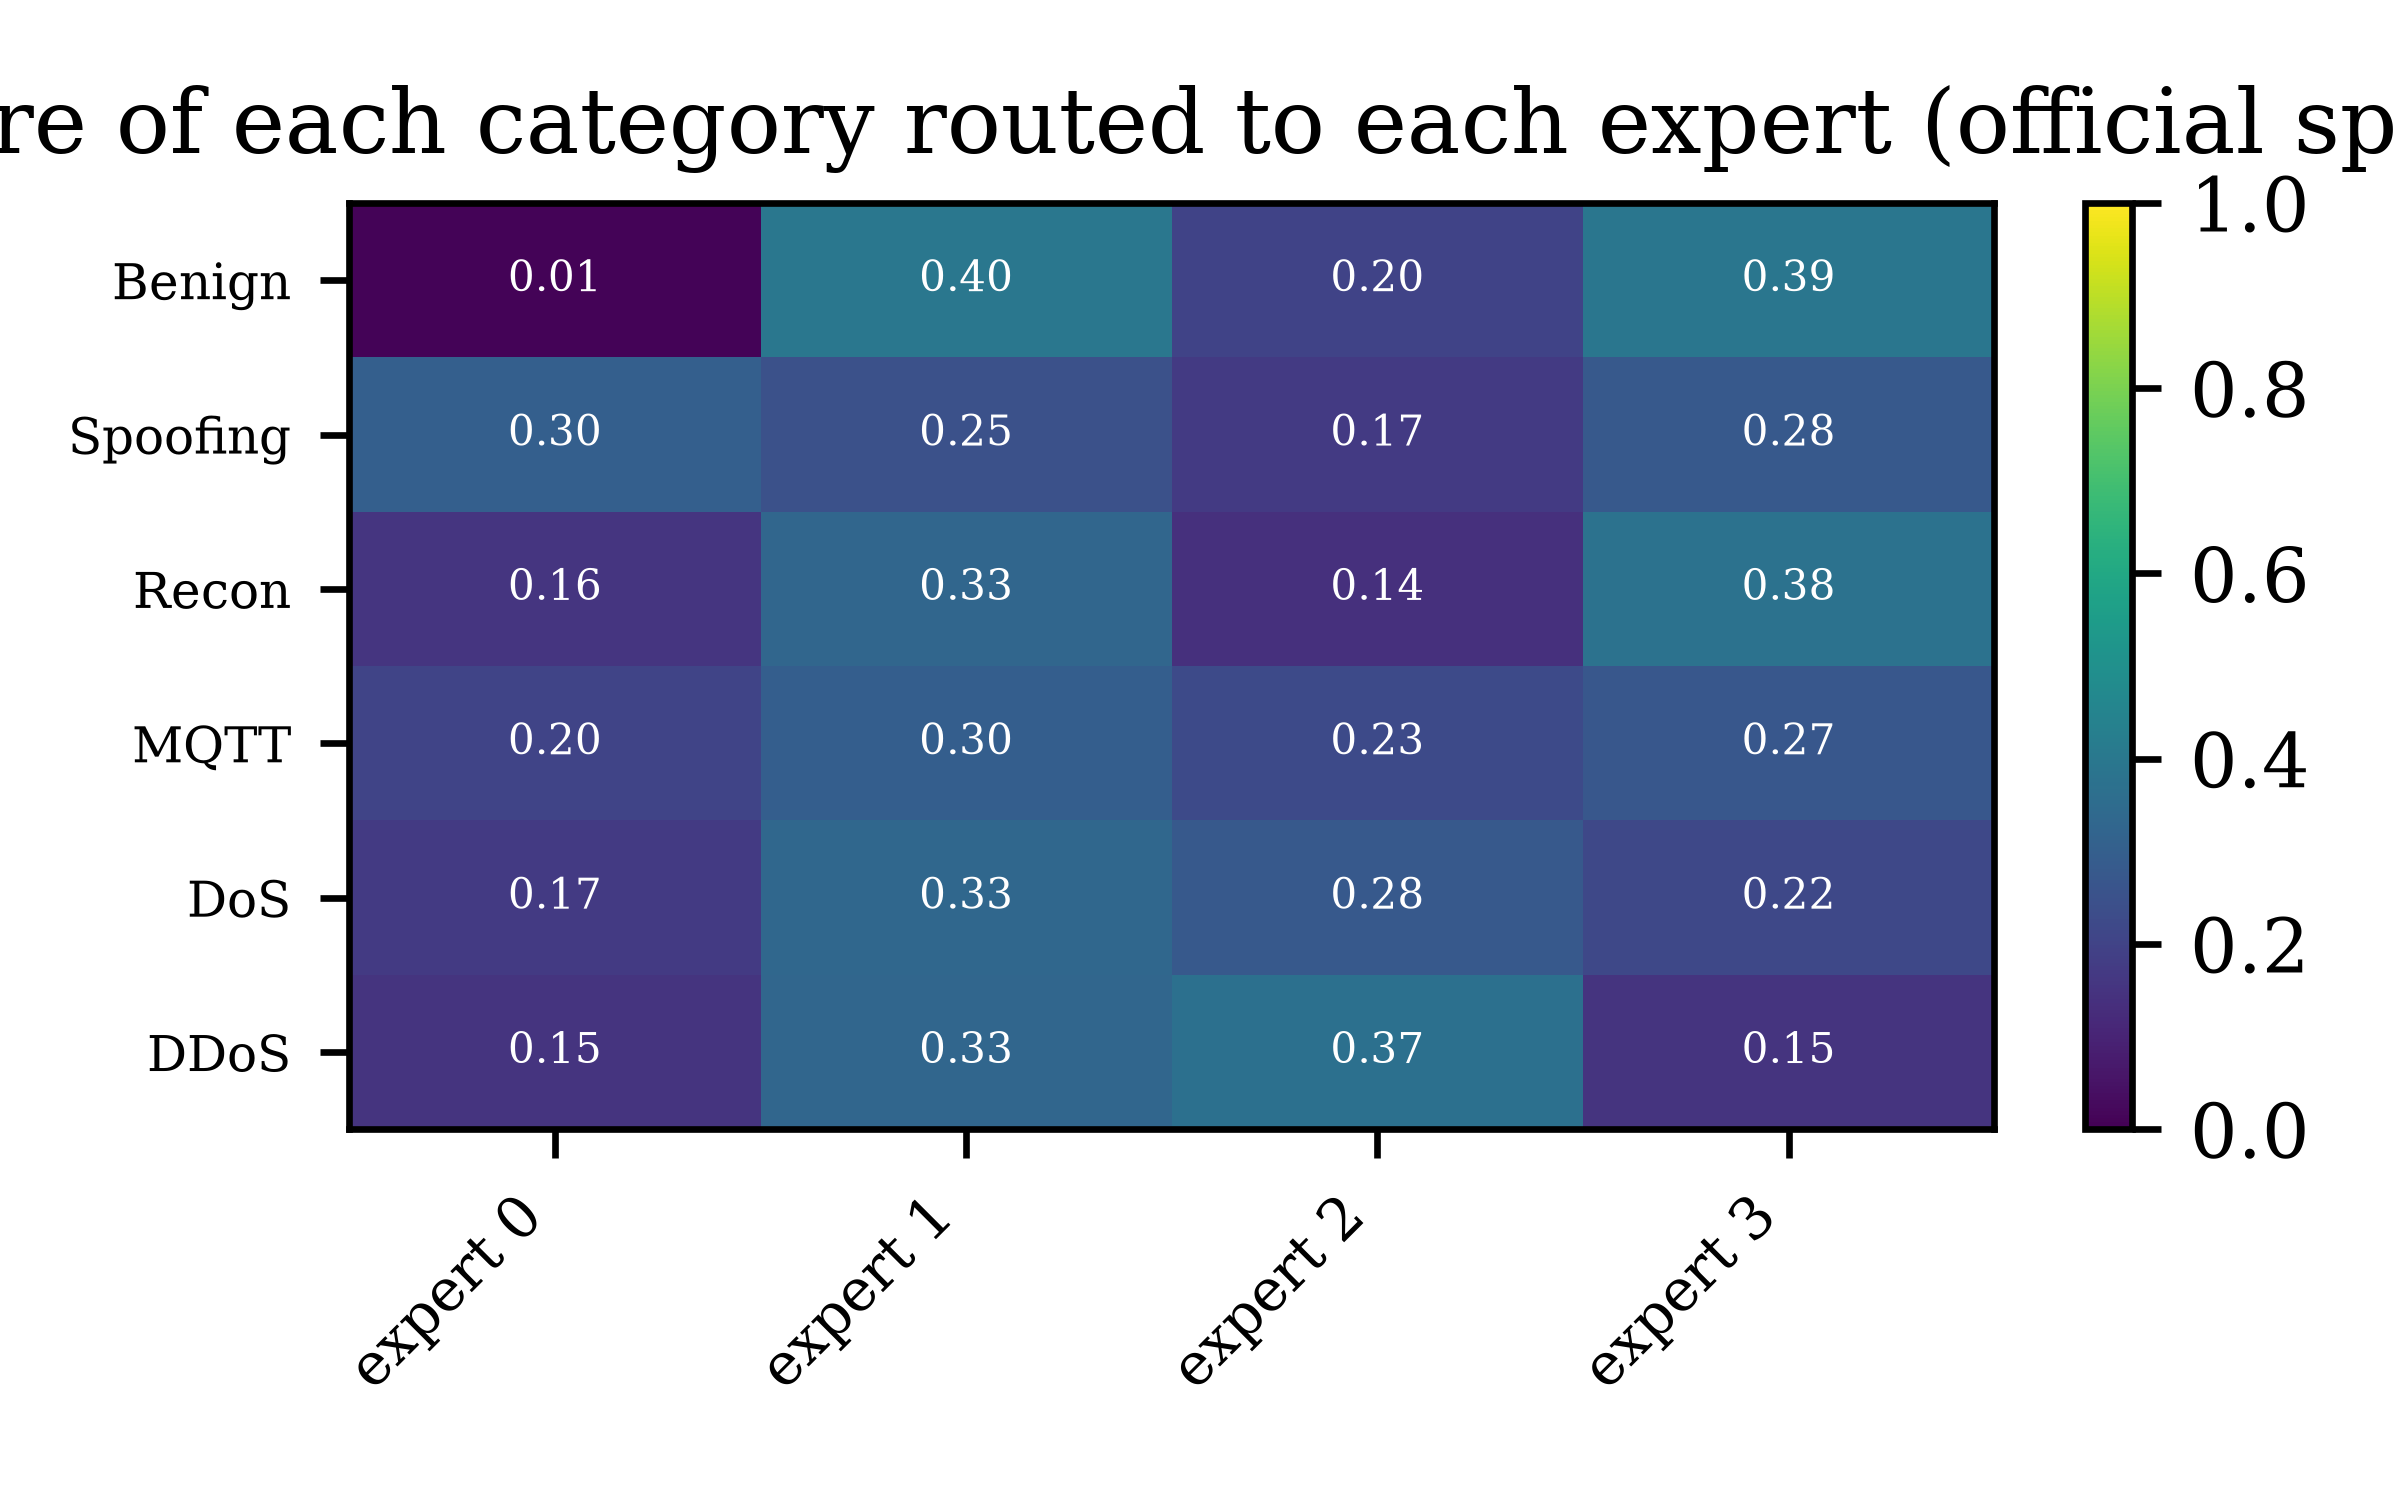
\includegraphics[width=0.9\textwidth]{figures/expert_by_category_official.png}
\caption{Share of each attack category sent to each expert, mean of 5 seeds, official split.}
\label{fig:6}
\end{figure}

Table 9 reports the per-seed expert specialisation (NMI) and routing load across all four experts, and Figure 6 visualises the resulting category-level routing shares. The four experts do not specialise strongly by attack category under 5 seeds. NMI(expert, 6-category label) = 0.1911 is well below the 0.5 threshold set out in H5; NMI(expert, 19-class label) = 0.5132 is near the threshold. Hypothesis H5 is therefore not supported, and we report this honestly rather than fitting a different seed subset. The per-category routing (Figure 6) shows a more diffuse pattern than a single-seed configuration suggested in an earlier draft: each expert receives 15 to 33\% of the test traffic and no expert claims any single category. Nonetheless, the Wilcoxon result of Section 5.2 shows the MoE head still raises per-class macro-F1 over every deep baseline, so the mixture adds representational capacity even without clean category-level specialisation. A follow-up with 6 experts (one per category) is listed in Section 6.2 Future Work.

A natural question is whether the three heads produce mutually consistent predictions at inference, given that the KL probability-aggregation loss trains for consistency without enforcing it. We computed, on all 5 seeds and over 1,584,389 official-split test windows per seed, (a) the rate at which the parent of the argmax 19-class prediction equals the argmax 6-category prediction and (b) the rate at which the parent of the argmax 6-category prediction equals the argmax binary prediction. Table 10 reports both plus the joint consistency rate.

\begin{table}[htbp]
\centering
% Source: tables/hierarchy_consistency.csv (no LaTeX export available; see traceability.json)
\caption{Hierarchy consistency at inference, official split, mean +/- std over 5 seeds (B1 review analysis).}
\label{tab:10}
\end{table}

TRACE-MoE has the highest joint hierarchy-consistency rate of any model (99.913 +/- 0.023\%), followed by TF-SAGE-lite (99.908), Transformer (99.805), random forest (99.749) and BiLSTM-DNN (99.598). The KL probability-aggregation term therefore produces hierarchically-coherent predictions in the overwhelming majority of windows (only about 0.09\% of windows have inconsistent 19 / 6 / 2-class argmaxes for TRACE-MoE), without any explicit constrained decoding at inference. For a hospital-gateway deployment where a single forward pass yields a binary alert, a category label and a fine class, this is operationally desirable.

\subsection{Calibrated abstention (RQ3)}
The AURC column is computed on temperature-calibrated 19-class softmax (per-seed temperature T grid-fitted on validation NLL, Guo et al. 2017 [31]); this is why Table 11's AURC values differ from the raw-softmax AURC in Table 12.

\begin{table}[htbp]
\centering
\begin{table}[htbp]
\centering
\caption{Abstain layer: coverage, error with and without abstention, AURC and calibration. [Report T14; source: results\_v2/tables/abstain\_official.csv]}
\label{tab:abstain_official}
\begin{tabular}{lcccccccccc}
\toprule
model & n\_seeds & coverage & risk\_full & selective\_risk & aurc & accepted\_macro\_f1 & ece\_raw & ece\_calibrated & source\_runs & source\_git\_commits \\
\midrule
rf & 5 & 87.26 $\pm$ 0.31 & 0.64 $\pm$ 0.07 & 0.02 $\pm$ 0.00 & 0.03 $\pm$ 0.01 & 92.06 $\pm$ 0.21 & 1.77 $\pm$ 0.34 & 0.51 $\pm$ 0.11 & rf\_official\_T1\_seed42|rf\_official\_T1\_seed43|rf\_official\_T1\_seed44|rf\_official\_T1\_seed45|rf\_official\_T1\_seed46 & no-git \\
transformer & 5 & 95.70 $\pm$ 0.32 & 1.23 $\pm$ 0.14 & 0.60 $\pm$ 0.08 & 1.15 $\pm$ 0.55 & 81.49 $\pm$ 1.76 & 0.71 $\pm$ 0.07 & 0.69 $\pm$ 0.08 & transformer\_official\_T16\_seed42|transformer\_official\_T16\_seed43|transformer\_official\_T16\_seed44|transformer\_official\_T16\_seed45|transformer\_official\_T16\_seed46 & no-git \\
bilstm\_dnn & 5 & 96.26 $\pm$ 0.32 & 2.18 $\pm$ 0.03 & 0.65 $\pm$ 0.09 & 1.43 $\pm$ 1.21 & 77.13 $\pm$ 0.98 & 1.76 $\pm$ 0.03 & 0.91 $\pm$ 0.27 & bilstm\_dnn\_official\_T16\_seed42|bilstm\_dnn\_official\_T16\_seed43|bilstm\_dnn\_official\_T16\_seed44|bilstm\_dnn\_official\_T16\_seed45|bilstm\_dnn\_official\_T16\_seed46 & no-git \\
trace\_moe & 5 & 95.78 $\pm$ 0.32 & 1.02 $\pm$ 0.05 & 0.65 $\pm$ 0.03 & 1.71 $\pm$ 0.76 & 82.38 $\pm$ 2.35 & 0.90 $\pm$ 0.04 & 0.52 $\pm$ 0.14 & trace\_moe\_official\_T16\_seed42|trace\_moe\_official\_T16\_seed43|trace\_moe\_official\_T16\_seed44|trace\_moe\_official\_T16\_seed45|trace\_moe\_official\_T16\_seed46 & no-git \\
tfsage\_lite & 5 & 95.58 $\pm$ 0.39 & 1.30 $\pm$ 0.09 & 0.62 $\pm$ 0.11 & 2.03 $\pm$ 0.92 & 83.35 $\pm$ 1.45 & 1.18 $\pm$ 0.07 & 0.72 $\pm$ 0.07 & tfsage\_lite\_official\_T16\_seed42|tfsage\_lite\_official\_T16\_seed43|tfsage\_lite\_official\_T16\_seed44|tfsage\_lite\_official\_T16\_seed45|tfsage\_lite\_official\_T16\_seed46 & no-git \\
\bottomrule
\end{tabular}
\end{table}
\caption{Calibrated abstention layer, official split, 5 seeds.}
\label{tab:11}
\end{table}

\begin{figure}[htbp]
\centering
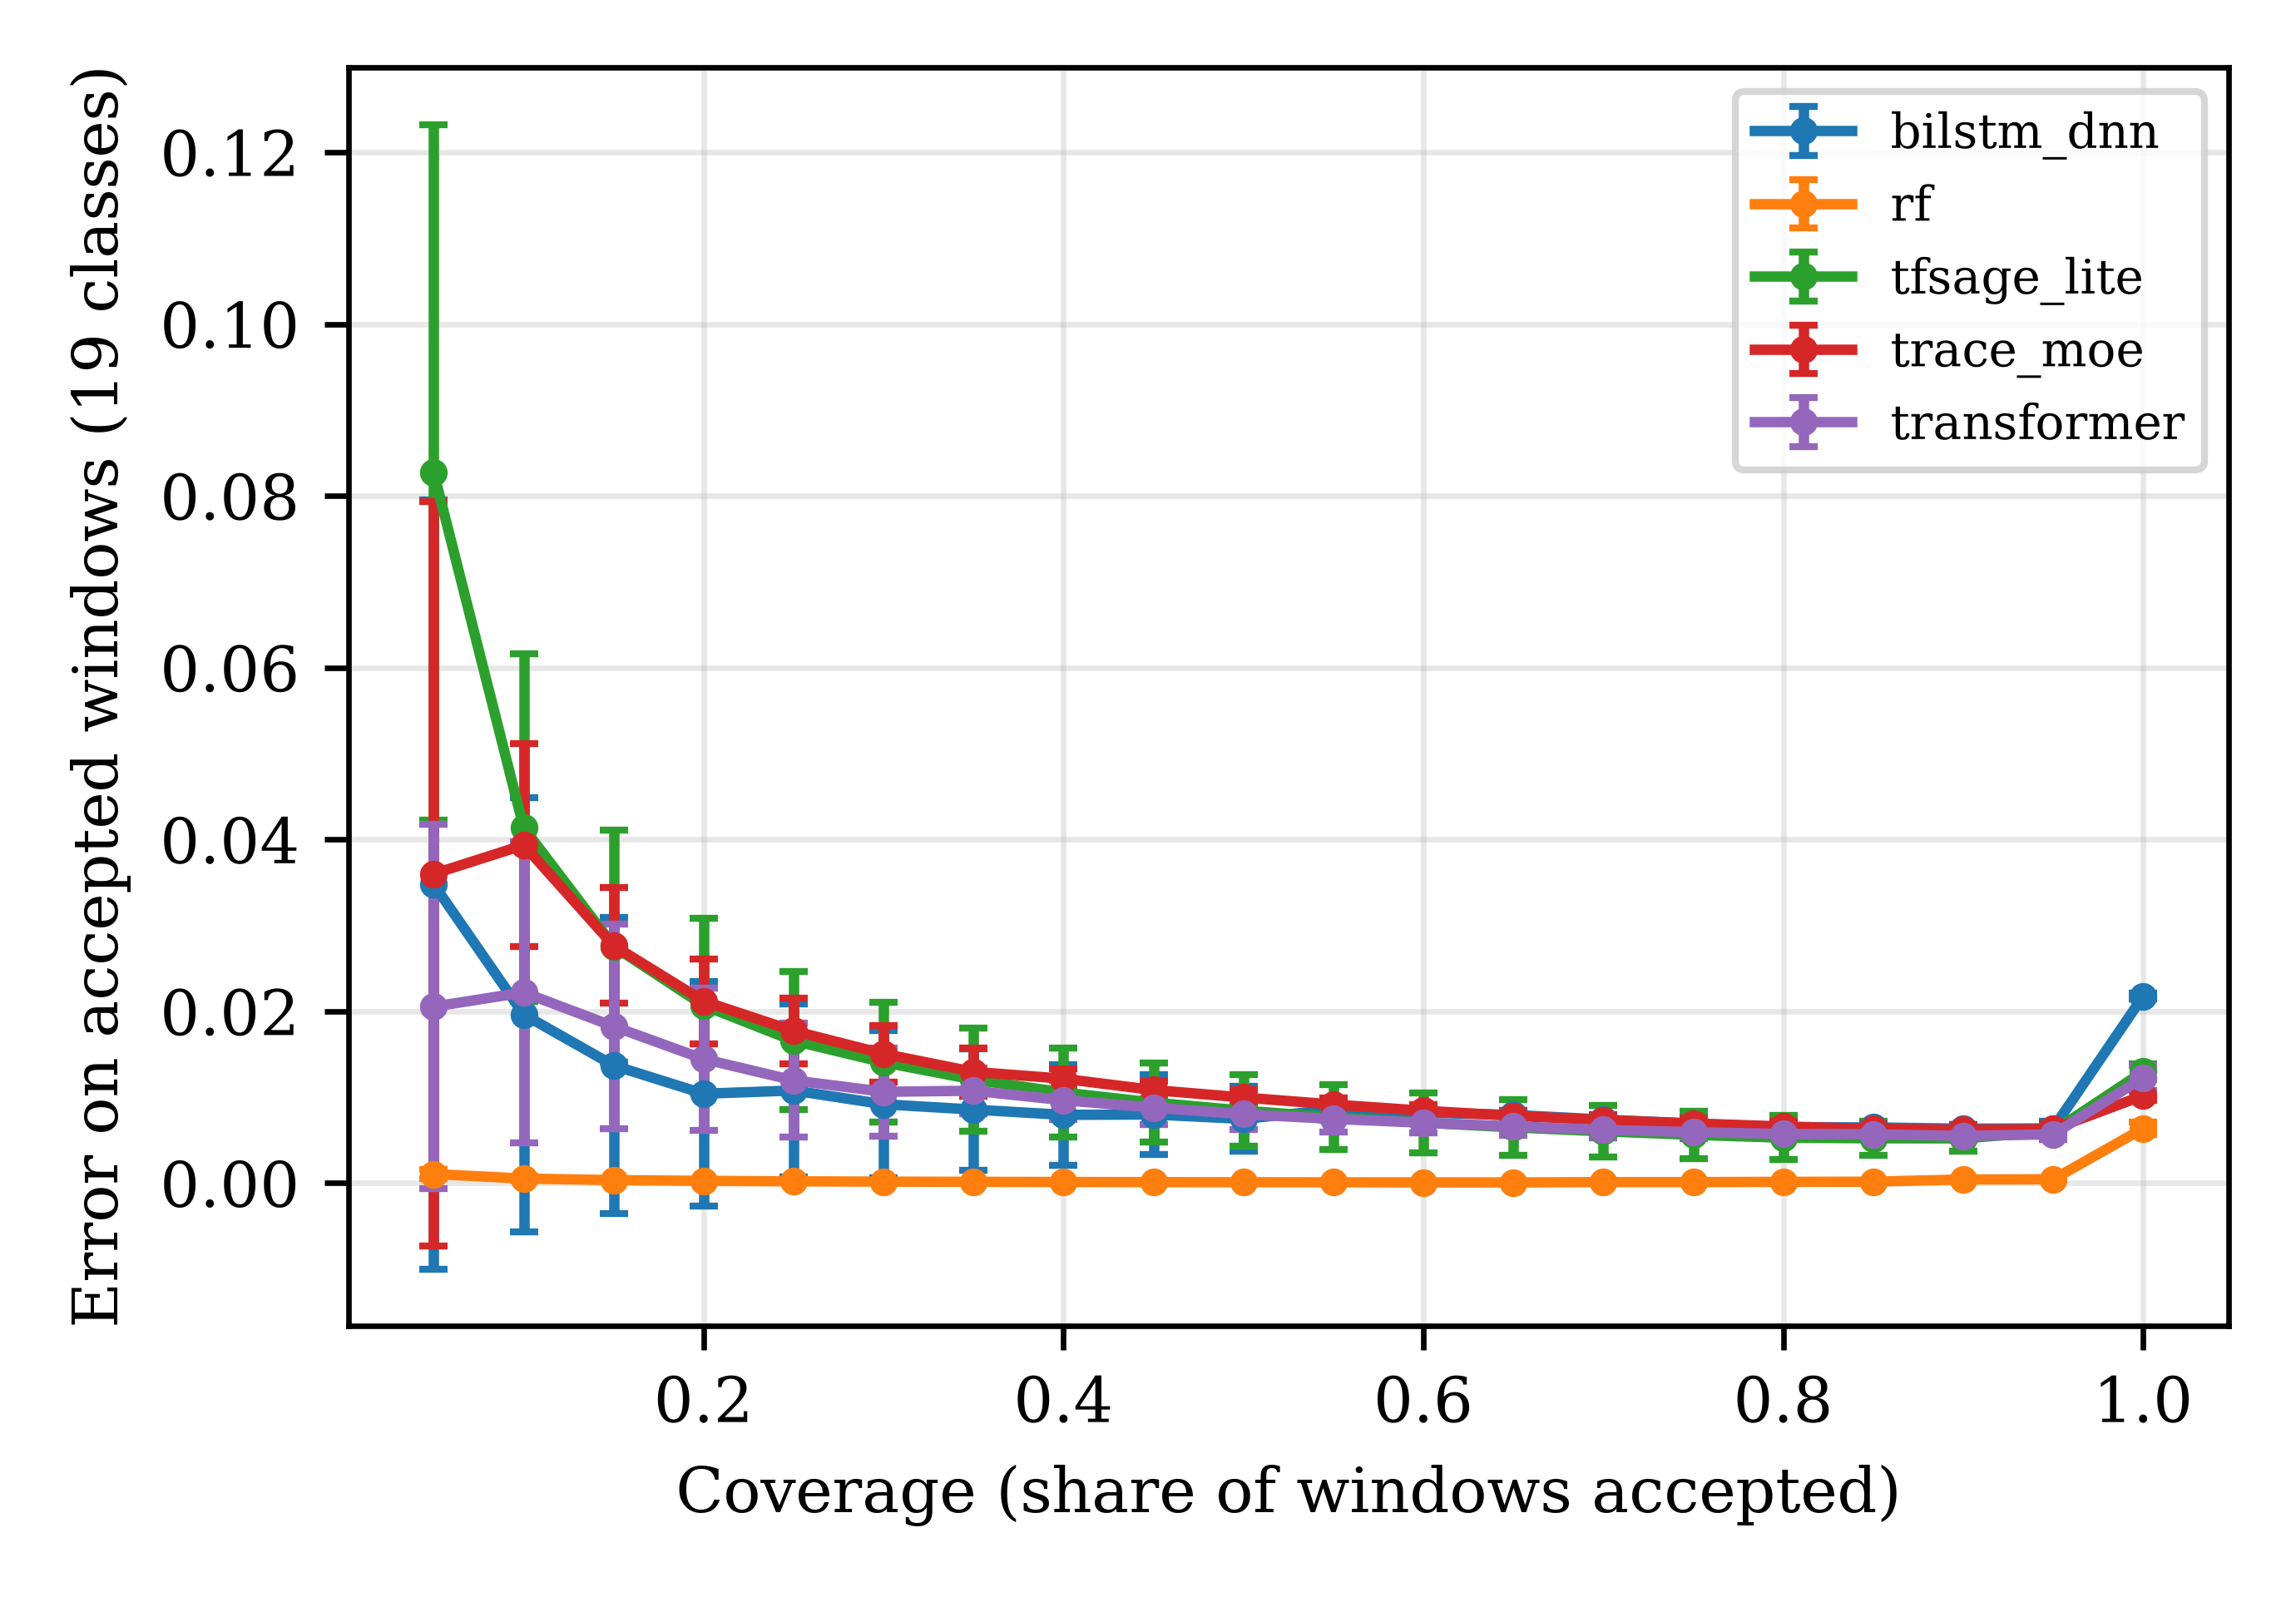
\includegraphics[width=0.9\textwidth]{figures/risk_coverage.png}
\caption{Risk-coverage curves of every model on the official split, mean of 5 seeds. Lower is better.}
\label{fig:7}
\end{figure}

At the validation-set threshold TRACE-MoE accepts 95.78 $\pm$ 0.32\% of test windows. Its error on the full test set is 1.02 $\pm$ 0.05\%, which drops to 0.65 $\pm$ 0.03\% on accepted windows (Table 11). The AURC is 1.71 $\pm$ 0.76\%, which places TRACE-MoE at rank 4 of 5: random forest leads at 0.03 $\pm$ 0.01\% by a wide margin, followed by Transformer and BiLSTM-DNN. Figure 7 plots the risk-coverage curves underlying these AURC values for all five models. Hypothesis H9 is not supported. ECE drops from 0.90 $\pm$ 0.04 raw to 0.52 $\pm$ 0.14 after temperature scaling, consistent with Transformer and with the general calibration literature [31]. The abstain layer is implemented, calibrated and transparent, but on CICIoMT2024 it does not displace random forest at AURC ranking; this is a legitimate limit of a deep window-level model competing with a tree ensemble whose single-flow confidence ranking is already very sharp. On accepted windows specifically, TRACE-MoE's selective risk (0.65\%) remains approximately 30 times random forest's (0.02\%) --- the gap on accepted traffic is of the same order as the gap on the full test set, so the abstention layer narrows error density but does not close the model-level gap on confidence-ranking quality (which is also why Table 12 shows that alternative scores like margin and negative entropy do not meaningfully alter the picture). This gap is a direct consequence of random forest's near-perfect confidence calibration on the dominant DDoS classes, which the sanity-check histogram above confirms (mean confidence 0.979 on correct predictions, 0.515 on wrong predictions); closing it is listed under Section 6.2 Future Work via ranking-improving scores (energy, Mahalanobis in representation space, selective conformal prediction).

We further examine whether ranking-improving confidence scores (margin, negative entropy) can lower AURC beyond temperature-scaled max-softmax, since selective-classification theory suggests that monotone post-hoc calibration cannot change confidence rankings and therefore cannot change AURC. We re-ran AURC on the saved test logits with three scores: max-softmax (our baseline, equivalent to the value in Table 11 up to the abstain-layer threshold), margin (p\_top1 - p\_top2), and negative entropy (sum p * log p, higher = more confident). Table 12 reports the result across all 5 seeds and 5 models.

\begin{table}[htbp]
\centering
% Source: tables/alt_aurc.csv (no LaTeX export available; see traceability.json)
\caption{Alternative confidence scores for AURC on the official split, mean +/- std over 5 seeds.}
\label{tab:12}
\end{table}

All three AURC values here are computed on RAW (uncalibrated) 19-class softmax; the AURC in Table 11 is on temperature-calibrated softmax. For TRACE-MoE the raw max-softmax AURC (1.456\%) is slightly lower than the calibrated AURC in Table 11 (1.71\%), consistent with the selective-classification result that monotone post-hoc calibration cannot change confidence ranking (so should not change AURC in expectation) but a per-seed grid-searched temperature does add variance (std 0.76 vs 0.116).

For TRACE-MoE, margin and negative-entropy both lower AURC by less than one hundredth of a percentage point relative to max-softmax (1.456 -> 1.448 and 1.449). For BiLSTM-DNN and TF-SAGE-lite the alternative scores save a few hundredths; for Transformer the saving is slightly larger (-0.04 pt for margin) but the ranking across models does not change: random forest remains almost two orders of magnitude ahead on AURC regardless of the score. This is consistent with the theoretical point raised by the reviewer: for a well-trained deep model, the three scores encode almost the same ranking of samples, so AURC is effectively a property of the model, not the score. Ranking-improving alternatives (energy, Mahalanobis-in-representation-space, selective conformal prediction, ensemble variance) that break out of this family are listed as Future Work.

As a sanity check on the random-forest AURC result, we examined the saved RF probabilities (sklearn's predict\_proba, which is the normalised share of trees voting for each class in a 200-tree class-balanced ensemble). The mean max-softmax confidence on correct predictions is 0.979 and on wrong predictions is 0.515, averaged over 5 seeds. Of about 1,540,000 correctly classified test windows per seed, 86.5\% fall in the [0.9, 1.0] confidence bin while only about 450 incorrectly classified windows do; the mean per-seed error rate on the full test set is 0.63\%. The large separation between confident-correct and confident-wrong populations is what drives RF's near-zero AURC, not an implementation bug; a histogram of the per-bin counts for all 5 seeds is in results\_v2/tables/rf\_confidence\_histogram.csv.

\subsection{Efficiency (RQ4)}
\begin{table}[htbp]
\centering
\begin{table}[htbp]
\centering
\caption{Model size and latency. [Report T15; source: results\_v2/efficiency/efficiency.csv]}
\label{tab:efficiency}
\begin{tabular}{lccccccccccc}
\toprule
model & T & params & size\_mb\_fp32 & cpu\_bs1\_ms\_per\_window & cpu\_bs1\_windows\_per\_s & cpu\_bs1024\_ms\_per\_window & cpu\_bs1024\_windows\_per\_s & cuda\_bs1\_ms\_per\_window & cuda\_bs1\_windows\_per\_s & cuda\_bs1024\_ms\_per\_window & cuda\_bs1024\_windows\_per\_s \\
\midrule
bilstm\_dnn & 16 & 70811 & 0.27 & 3.733 & 267.9 & 0.0265 & 37690.5 & 0.3817 & 2620.2 & 0.0037 & 269101.9 \\
transformer & 16 & 308251 & 1.176 & 1.1627 & 860.1 & 0.0332 & 30127.6 & 0.7461 & 1340.4 & 0.0079 & 125921.5 \\
tfsage\_lite & 16 & 109723 & 0.419 & 0.9362 & 1068.1 & 0.0155 & 64522.4 & 1.0585 & 944.7 & 0.0036 & 275032.2 \\
trace\_moe & 16 & 685041 & 2.613 & 3.6253 & 275.8 & 0.0839 & 11914.3 & 2.3946 & 417.6 & 0.0151 & 66240.6 \\
\bottomrule
\end{tabular}
\end{table}
\caption{Model size and inference latency (single-thread CPU; RTX 3050 Laptop GPU for CUDA).}
\label{tab:13}
\end{table}

Table 13 reports the model size and inference latency for every model. TRACE-MoE has 685,041 parameters (2.613 MB in fp32), which fits within the 5 M-parameter edge budget. On a single CPU thread it runs at 0.0839 ms per window at batch 1024 and 3.6253 ms at batch 1. The Transformer is faster at batch 1024 (0.0332 ms per window) despite having 0.308 M parameters because the MoE router adds an argmax hop; TF-SAGE-lite is faster still (0.0155 ms per window) because of its lighter graph aggregation. H10 is partly supported: TRACE-MoE fits an edge gateway, but it is not the fastest deep model.

Operational use in a hospital SOC. The hierarchical heads and the calibrated abstention are designed to slot into a Security Operations Centre workflow as follows. A window produces, in a single forward pass, (i) a binary alert at the L2 head, (ii) a category label at the L6 head useful for playbook routing (DoS or DDoS alerts go to network engineering, Recon alerts to threat hunting, MQTT alerts to the device-management team) and (iii) a fine class at the L19 head for forensic context. Table 10 shows that the three outputs agree on about 99.9\% of windows for TRACE-MoE, so the SOC does not need a reconciliation step. Windows below the 95\%-coverage calibrated threshold are abstained from and placed on a 'needs review' queue rather than silently dropped, which (per Table 11) carries the error rate on accepted windows down from 1.02\% to 0.65\% at the cost of about 4\% of the throughput landing on human triage.

\section{Limitations and Future Work}
\subsection{Limitations}
The study uses the Wi-Fi/MQTT part of CICIoMT2024 only; Bluetooth Low-Energy traffic is left to future work.

Each CICIoMT2024 file contains a single class, so windows never mix benign and attack traffic; detection of transitions inside a window is not evaluated.

Published-result comparisons (Table 8) use the authors' own splits and metrics and are therefore informational, not head-to-head.

Minimum class recall at 19 classes (10.52 \%) remains well below random forest's (20.06 \%); rare classes such as Recon-VulScan and MQTT-DDoS-Publish\_Flood would benefit from a per-class temperature or a rejection rule anchored at the minimum class.

The abstain layer is calibrated with temperature scaling but does not beat random forest in AURC (TRACE-MoE 1.71 \% vs RF 0.03 \%); alternative abstention scores (energy, Mahalanobis) are not evaluated.

Expert routing does not specialise at the attack-category level under 5 seeds (NMI = 0.1911). The paper is transparent about this.

\subsection{Future Work}
Four experiments were scoped and partly engineered but have not been executed on real CICIoMT2024 data. We list them so follow-up work can start from a documented baseline. The corresponding scripts are included in the released repository.

MoE-vs-dense ablation (H4). scripts/05\_ablation.py trains a dense feed-forward expert of the same parameter count as the MoE expert layer and compares 19-class macro-F1 on the official split with 5 seeds.

Feature-constrained adversarial robustness (H6). scripts/06\_robustness.py runs a 20-step projected gradient descent attack [38] on the 18 mutable flow features (timing and size statistics) within an L\_inf budget epsilon in \{0.05, 0.1, 0.25, 0.5\} in scaled units, enforcing non-negativity in raw units, reports the attack success rate per class, and tests black-box transfer across all five models.

Adversarial fine-tuning clean cost (H7). The same script also fine-tunes every neural model adversarially for 3 epochs on a 50/50 clean+PGD mix and measures the clean 19-class macro-F1 after adversarial fine-tuning.

Leave-one-attack-out open-set detection (H8). scripts/07\_unknown\_attacks.py removes one of the 18 attack classes at a time from training and measures the AUROC of the energy score [39] of the 19-class head at detecting the held-out class, compared with the AUROC of the max-softmax confidence.

Expert-count sensitivity. Train TRACE-MoE with 2, 6 and 8 experts to probe whether a per-category expert count improves routing NMI without sacrificing the current per-class Wilcoxon wins.

Bluetooth-Low-Energy intrusion detection. Extend the pipeline from Wi-Fi/MQTT flows to BLE snoop logs and the attacks catalogued in Table 4 of [1].

Beyond the four experiments above, we have identified further ablations and probes that would strengthen the paper but require retraining or new inference passes with modified forward graphs:

Top-1 vs top-2 routing. Compare the top-1 gate used here against top-2 routing (two experts active per window with normalised gate weights), measuring the macro-F1 lift against the extra inference cost.

Protocol-feature dependence. Mask the Protocol-Type feature inside the router (and separately inside the encoder) at inference and re-measure 19-class macro-F1 and the Wilcoxon result; this probes how much of TRACE-MoE's advantage depends on the protocol token versus the window structure.

Windowed tree baselines. Add LightGBM and XGBoost on single flows and a windowed-aggregation random forest (voting over the 16 last-flow predictions within each window, and a pooled-features variant) to normalise the input-granularity gap between RF and the deep models.

Ranking-improving abstention scores. Evaluate energy-based scores [39], Mahalanobis distance in representation space and selective conformal prediction as alternatives to temperature-scaled max-softmax, extending the AURC analysis of Table 12.

End-to-end throughput including PCAP-to-feature extraction, under both streaming (batch 1) and batched (batch 1024) conditions, measured on a representative IoMT edge gateway.

Device-disjoint and session-disjoint splits within the official protocol, to probe spatial and temporal robustness beyond the file-level split already used here.

\section{Conclusion}
We presented TRACE-MoE, a protocol-routed Mixture-of-Experts detector with hierarchical 2/6/19 heads and a temperature-calibrated abstain layer, and evaluated it on the Wi-Fi/MQTT part of CICIoMT2024 under 5 seeds and two split protocols against random forest, BiLSTM-DNN, Transformer and TF-SAGE-lite. Primary findings: TRACE-MoE is Friedman rank 1 over 95 (class, seed) blocks and beats every deep baseline at Holm-corrected p < 0.0001 while trailing random forest by 2.88 pt macro-F1 (p = 0.52, not significant); it is non-inferior to random forest on binary detection (+2.419 pt, 95 \% CI [+2.007, +2.830]) and leads the 6-category level at 91.31 $\pm$ 1.68\%. A quantified split-inflation audit measures 5.67 to 15.96 pt of random-split inflation across models and justifies the file-based protocol. All code, configurations and SHA-256-verified result files are released. Adversarial robustness, leave-one-attack-out and MoE-vs-dense ablation are the subject of ongoing work (Section 6.2).

\subsection{Data Availability Statement: The data used in this study are openly available in the Canadian Institute for Cybersecurity (CIC) repository at https://www.unb.ca/cic/datasets/iomt-dataset-2024.html. The code, configurations, logs and SHA-256-verified result tables and figures that reproduce every number in this paper are released at https://github.com/sharmasudhir08/TRACE-MoE-CICIoMT2024.}
\subsection{Author Contributions: The authors confirm contribution to the paper as follows: Sudhir Kumar Sharma: Conceptualization; Methodology; Software; Formal analysis; Investigation; Data curation; Writing -- Original Draft; Writing -- Review \& Editing; Visualization; Supervision; Project administration. Sneha Vasishth contributions before submission; expected roles include Validation, Resources, and additional Writing -- Review. All authors have read and agreed to the published version of the manuscript.}
\subsection{Funding: This research received no external funding.}
\subsection{Ethics Approval: Not applicable.}
\subsection{Conflicts of Interest: The authors declare no conflict of interest.}
\section*{Declarations}
\paragraph{Data Availability Statement} The data used in this study are openly available in the Canadian Institute for Cybersecurity (CIC) repository at https://www.unb.ca/cic/datasets/iomt-dataset-2024.html. The code, configurations, logs and SHA-256-verified result tables and figures that reproduce every number in this paper are released at https://github.com/sharmasudhir08/TRACE-MoE-CICIoMT2024.

\paragraph{Author Contributions} The authors confirm contribution to the paper as follows: Sudhir Kumar Sharma: Conceptualization; Methodology; Software; Formal analysis; Investigation; Data curation; Writing -- Original Draft; Writing -- Review \& Editing; Visualization; Supervision; Project administration. Sneha Vasishth contributions before submission; expected roles include Validation, Resources, and additional Writing -- Review. All authors have read and agreed to the published version of the manuscript.

\paragraph{Funding} This research received no external funding.

\paragraph{Ethics Approval} Not applicable.

\paragraph{Conflicts of Interest} The authors declare no conflict of interest.

\bibliographystyle{unsrt}
\bibliography{references}
\end{document}